\newpage
\section{RESULTS AND DISCUSSION}

%%%%%%%%%%%%%%%%%%%%%%%%%%%%%%%%%%%%%%%%%%%%%%%%%%%%%%%%%%%%%%%%%%%%%%%%%%%%%%%%%%%%%%%%
%%%%%%%%%%%%%%%%%%%%%%%%%%%%%%%%%%%%%%%%%%%%%%%%%%%%%%%%%%%%%%%%%%%%%%%%%%%%%%%%%%%%%%%%
The results section is divided into three logical blocks. First, simulations of the neat polymer were performed to verify the force field and to determine the key properties of the polymer. Subsequently, a series of neat API simulations were performed. Then, simulations of mixtures of different API concentrations in polymer were performed to see the behavior of the mixtures.  

\subsection{Simulations of neat PLA}
\subsubsection{Structural properties}
First, the simulations from 2 initial states were done (fibrilar and globular). The Figure \ref{fig:linearni} shows an example of the shortest polymer in a fibrilar conformation state, whereas Figure \ref{fig:sbalene} displays globular conformations of chains containing 20 and 200 monomer units on the left and right, respectively. 

\begin{figure}[htb]
	\centering
	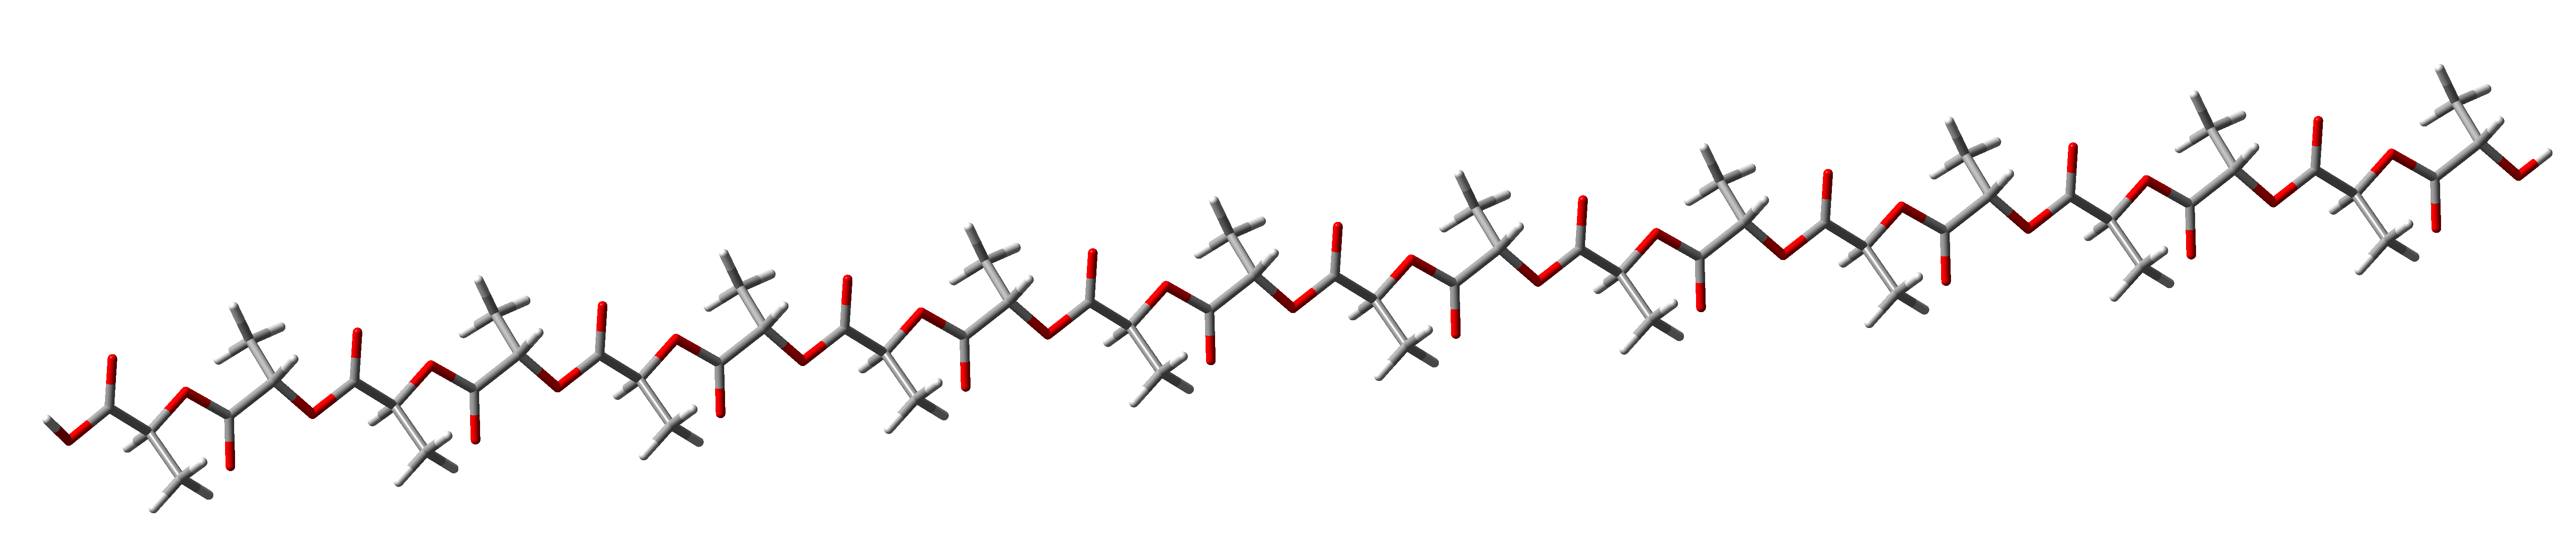
\includegraphics[width=0.9\linewidth]{img/pla_10d_tube.png}
	\caption{Fibrilar PLA polymer chain, 20 units}
	\label{fig:linearni}
\end{figure}

\begin{figure}[htb]
	\begin{subfigure}{0.5\textwidth}
		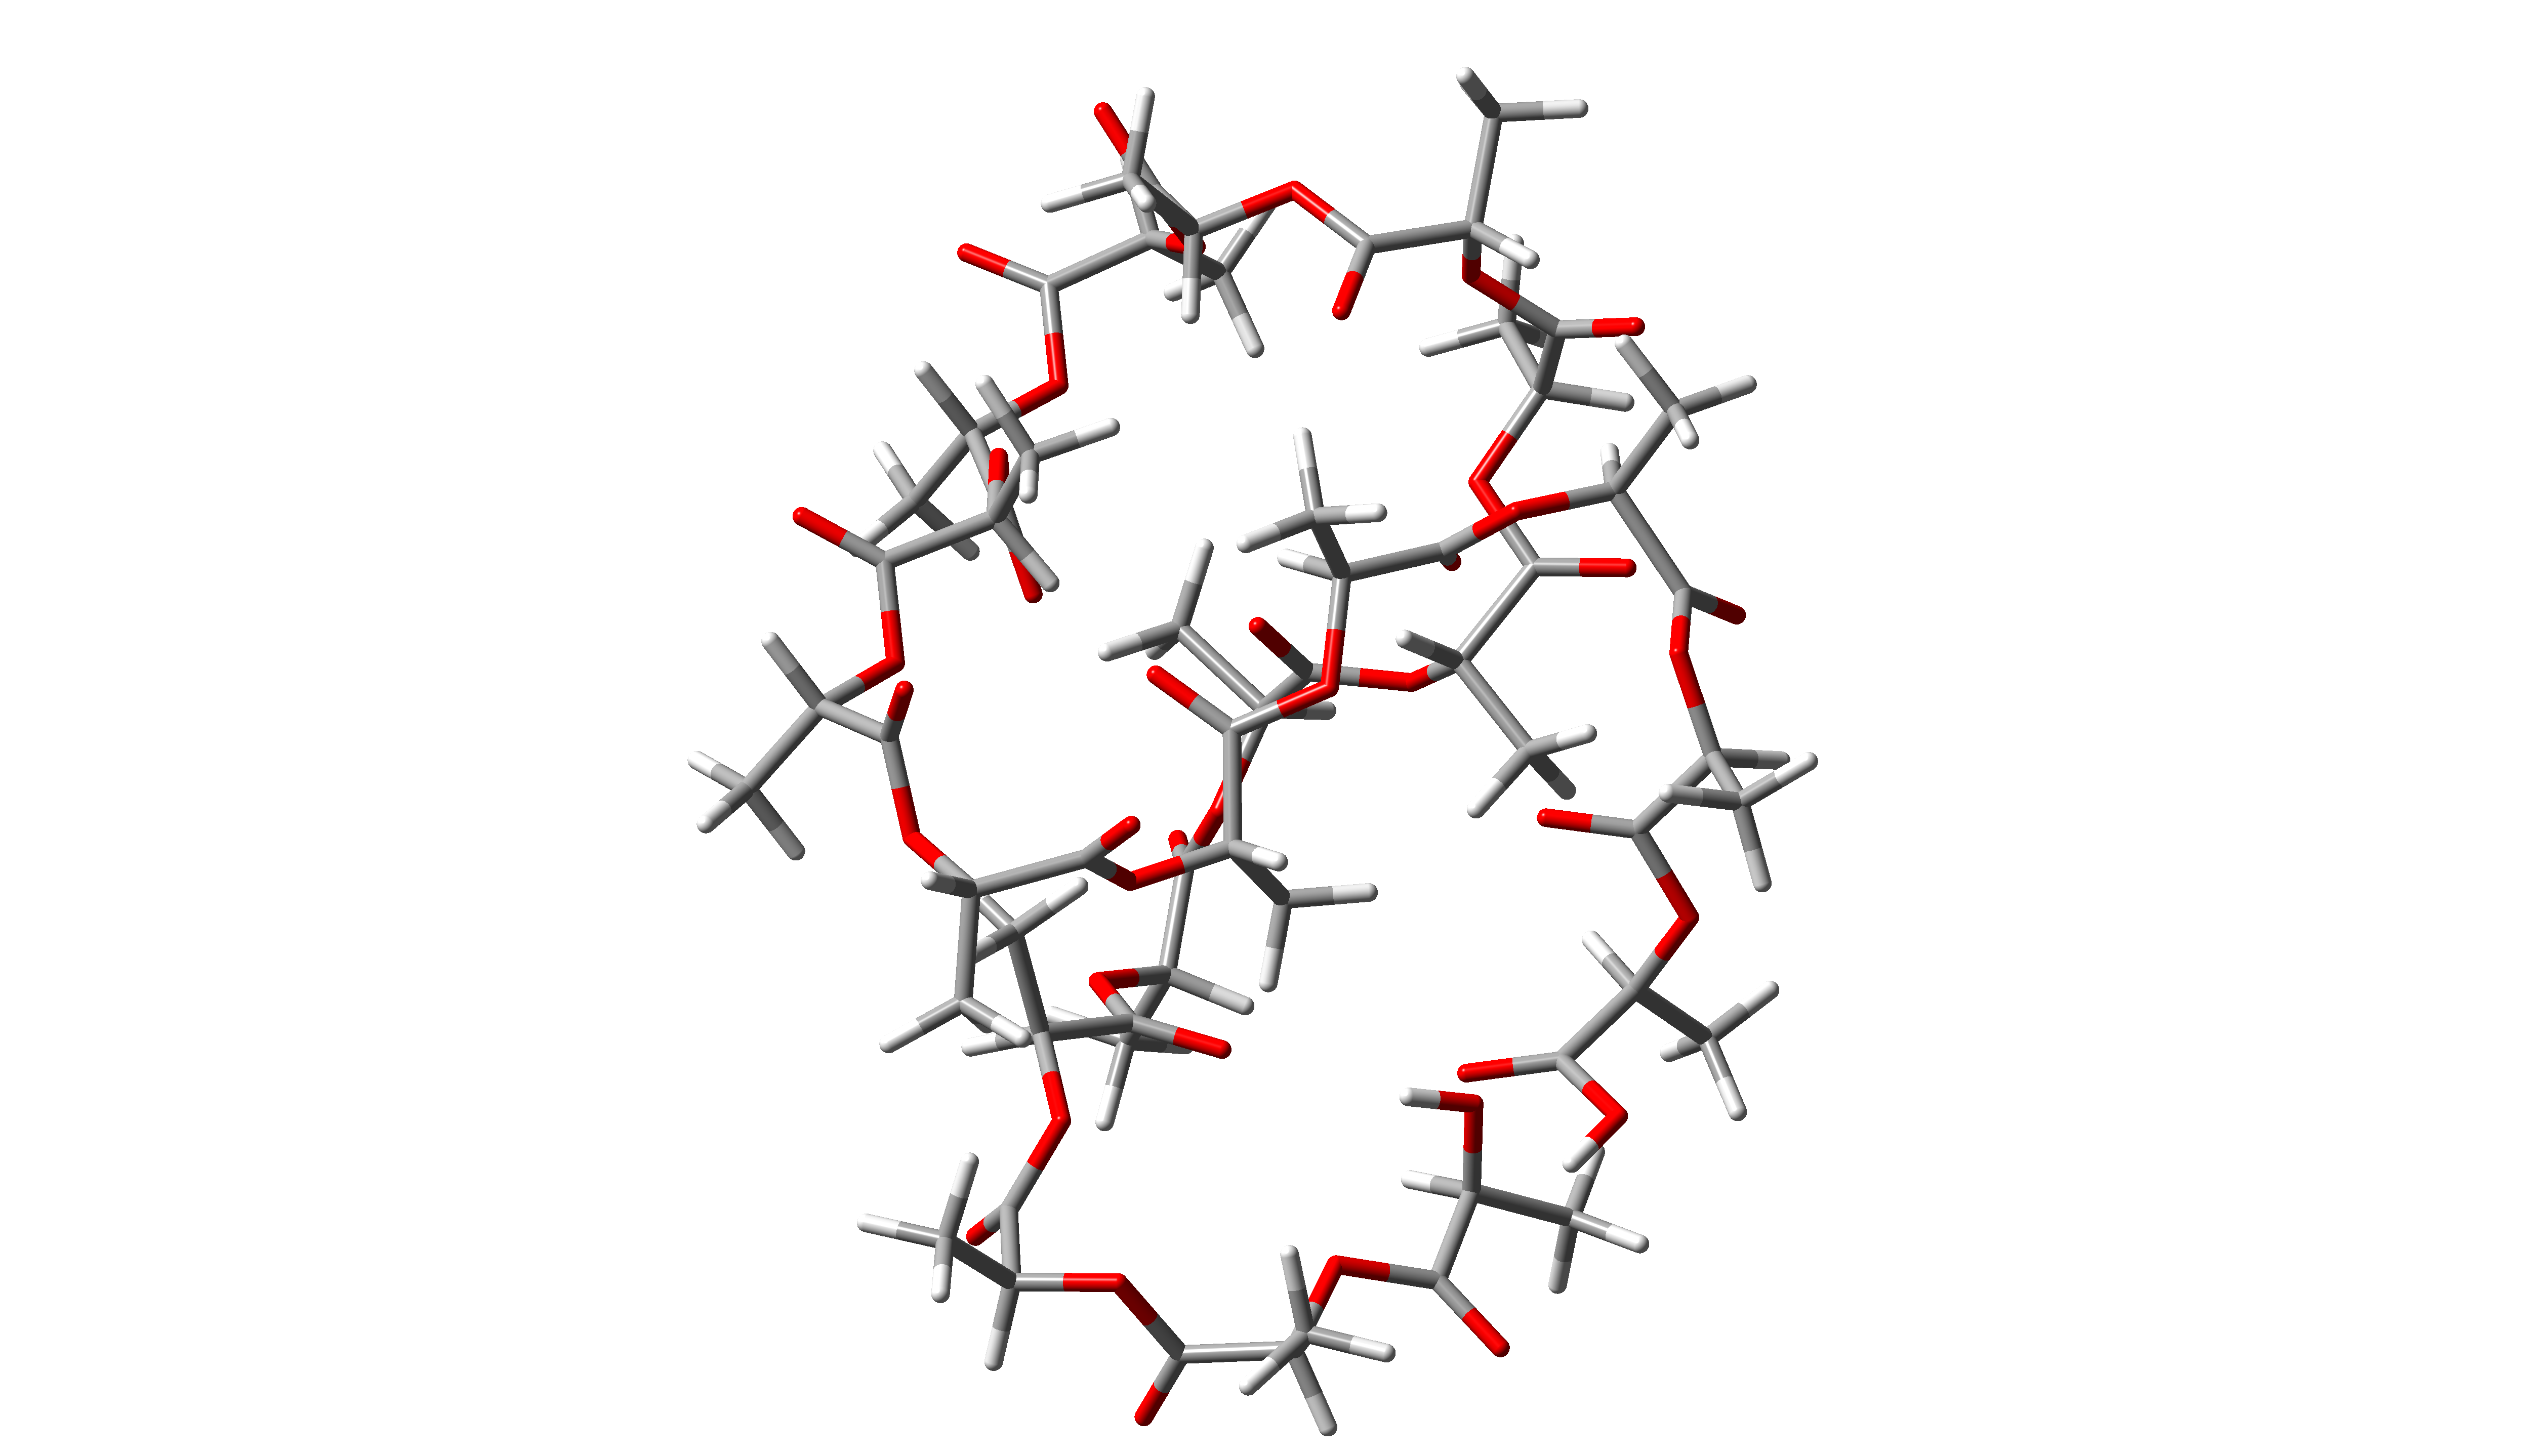
\includegraphics[width=0.9\linewidth]{img/pla_10g_tube.png} 
	\end{subfigure}
	\begin{subfigure}{0.5\textwidth}
		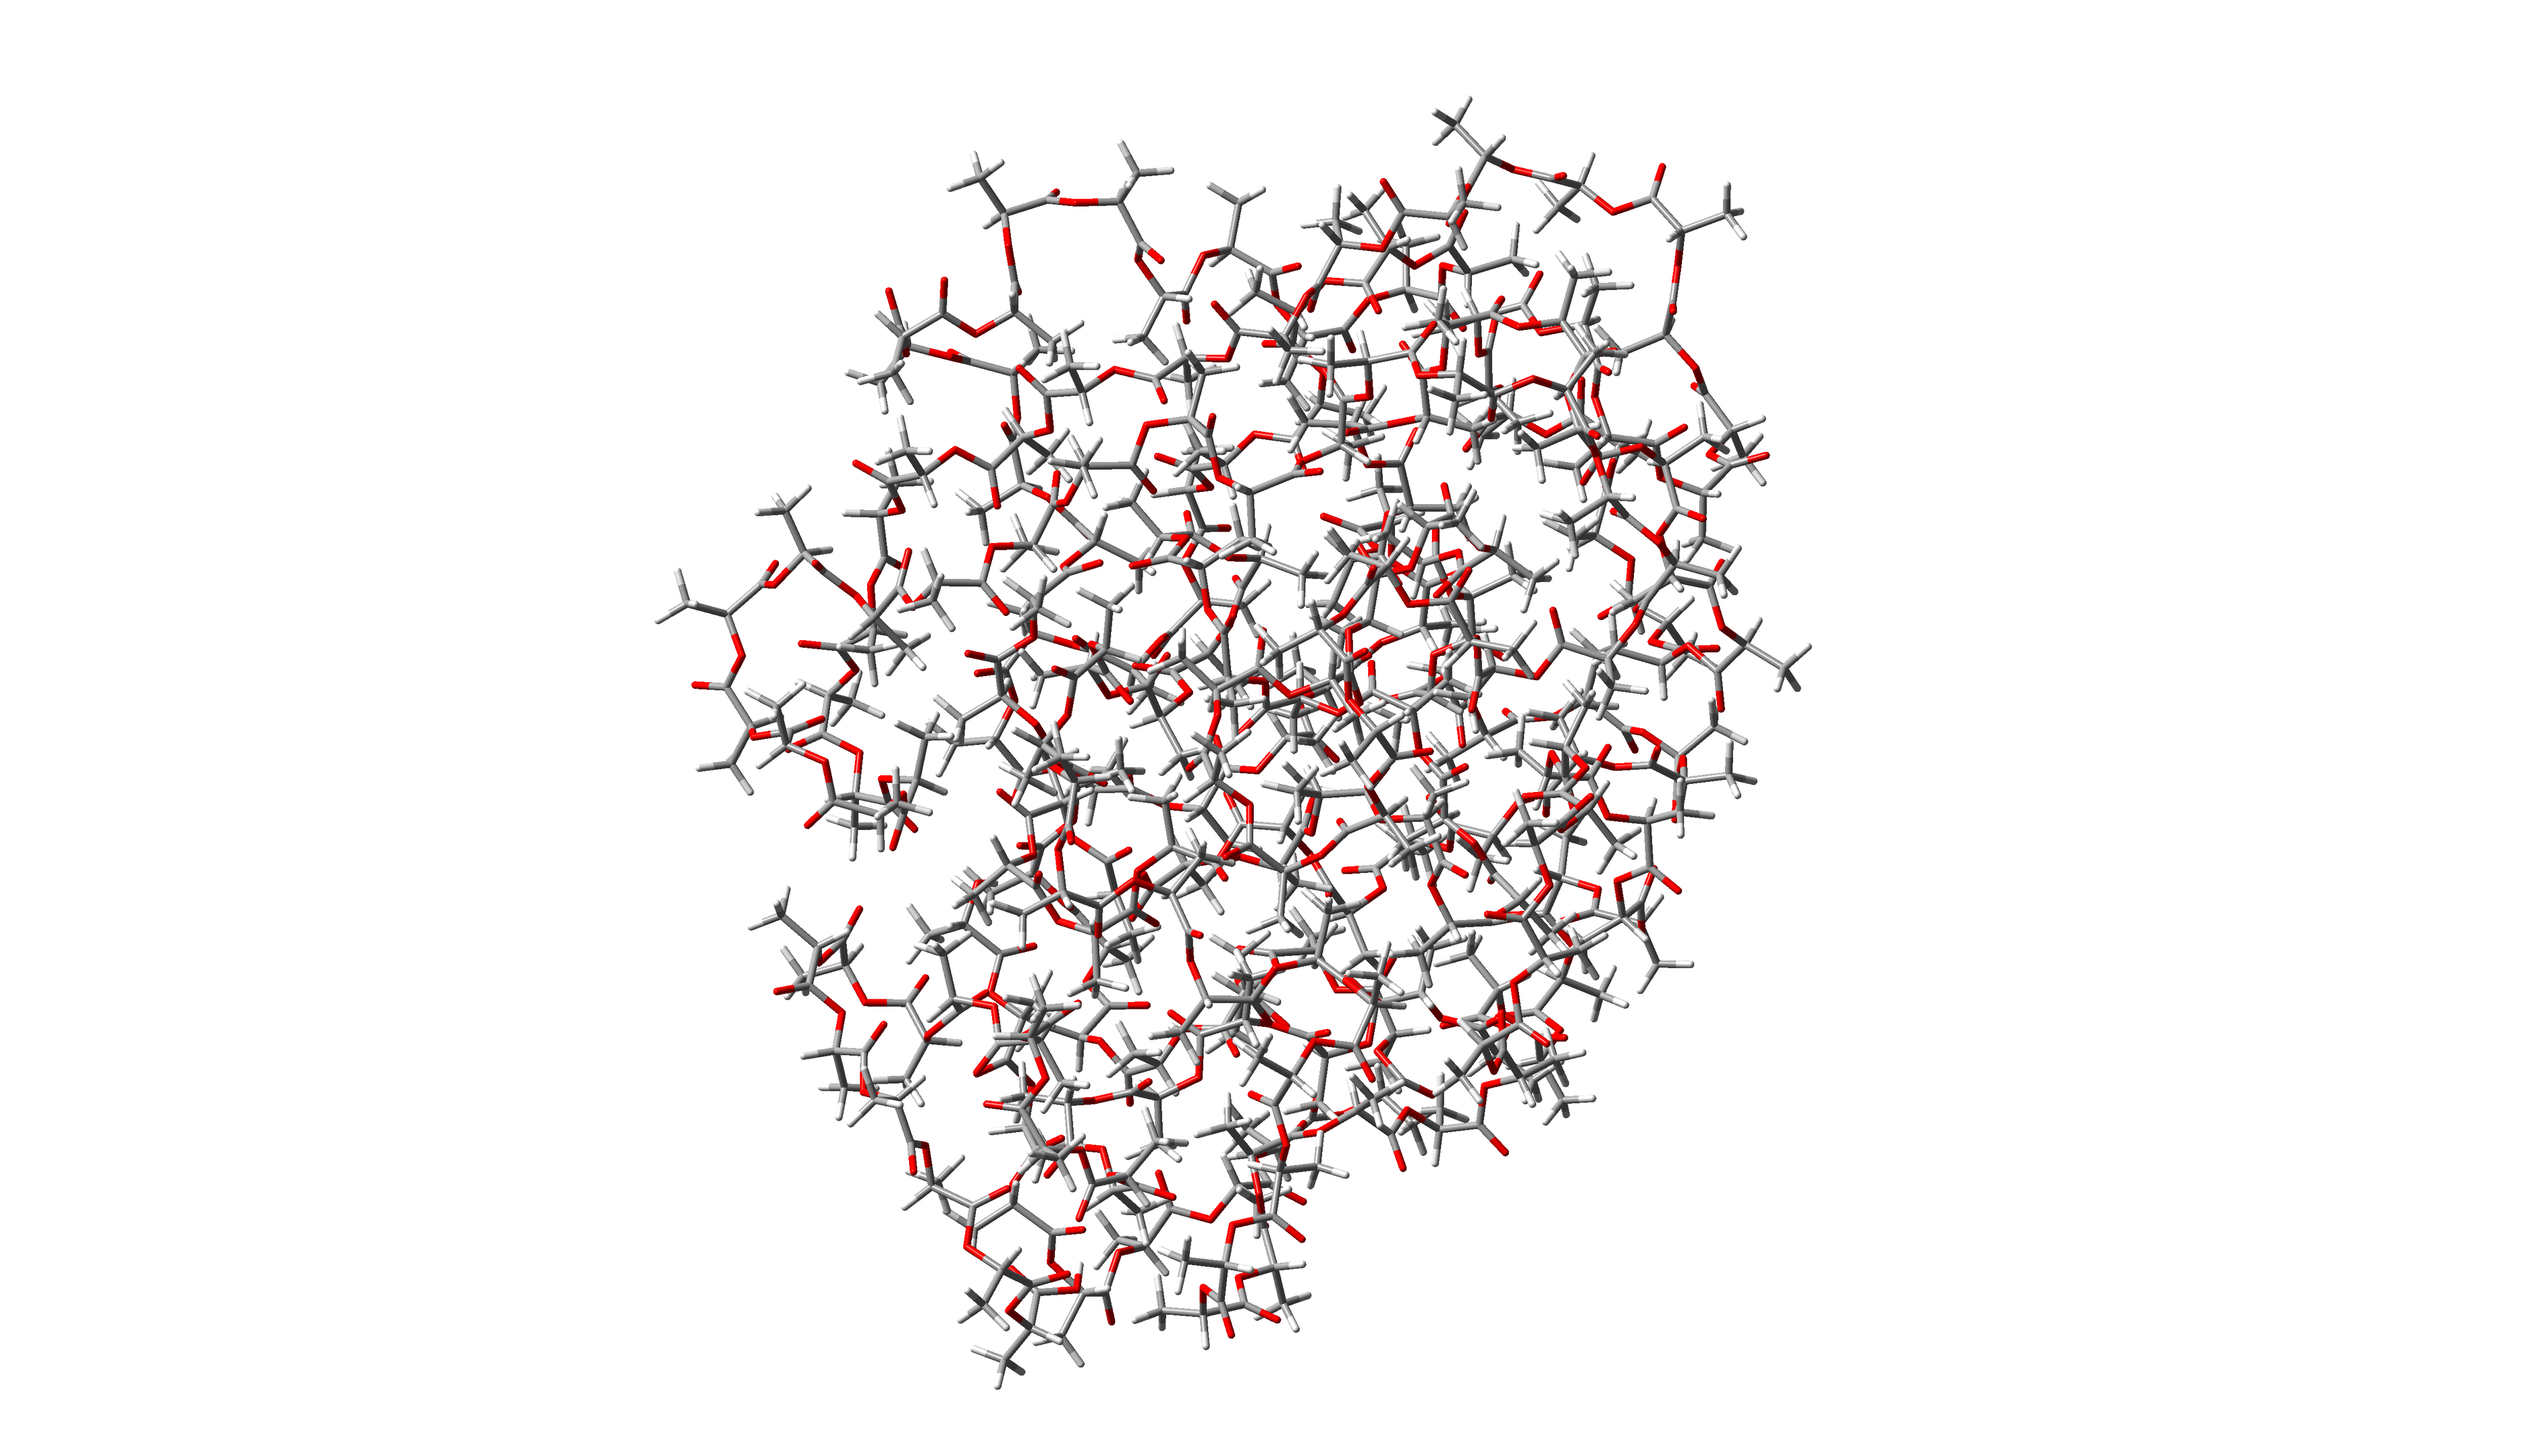
\includegraphics[width=0.9\linewidth]{img/pla_100g_tube.png} 
	\end{subfigure}   	
	\caption{Globular PLA polymer chain, 20 and 200 units}
	\label{fig:sbalene}
\end{figure}

To see the effects of initial conformations, molecular weight and thermal history of the polymer on bulk densities following simulations were performed. The design of the simulation boxes is in Table \ref{tab:pla_chains}. The simulations were first performed at the temperature of 500 K (run 1), then the box was heated up to 1000 K followed by re-cooling and simulating at a temperature of 500 K (run 2). All subsequent simulations were observing the system for 10~ns with a step 1 fs at 1 bar. From these simulations, the densities and the root mean square distance of the polymer chain termini with their standard deviations were evaluated.

\begin{table}[h]
	\centering
	\caption{Design of the neat PLA simulation boxes}
	\label{tab:pla_chains}
	\begin{tabular}{ccccc}
		\toprule
		\textbf{\boldmath$N_{\text{units}}$} & \textbf{\boldmath$n_{\text{chains}}$} & \textbf{\boldmath$N_{\text{atoms}}$} & \textbf{\boldmath$M$, g mol$^{-1}$} & \textbf{\boldmath$d$, \AA} \\
		\midrule
		20 & 140 & 25620 & 1459.3 & 67.9 \\
		40 & 70 & 25410 & 2900.5 & 67.7 \\
		60 & 40 & 24978 & 4341.8 & 64.3 \\
		80 & 35 & 25305 & 5783.1 & 67.7 \\
		100 & 28 & 25284 & 7224.3 & 67.7 \\
		120 & 23 & 24909 & 8665.6 & 67.3 \\
		140 & 20 & 25260 & 10106.8 & 67.6 \\
		160 & 17 & 24531 & 11548.1 & 67.0 \\
		180 & 15 & 24345 & 12989.4 & 66.8 \\
		200 & 14 & 25242 & 14430.6 & 67.6 \\
		\bottomrule
	\end{tabular}
\end{table}

The following graphical representation of the results (Figure \ref{fig:pla_hustoty}) shows a trend of an increasing density depending on the length of the chain (molecular weight), which is independent of the initial conformation of the molecule, the values differs only in . It is also visible that densities for longer chains converge to a constant value. From this finding, we can consider that a system above $M_\mathrm{w}$~=~9~000~$\mathrm{g \ mol^{-1}}$ has reached the polymer limit within the simulation.

\begin{figure}[htb!]
	\begin{subfigure}{0.5\textwidth}
		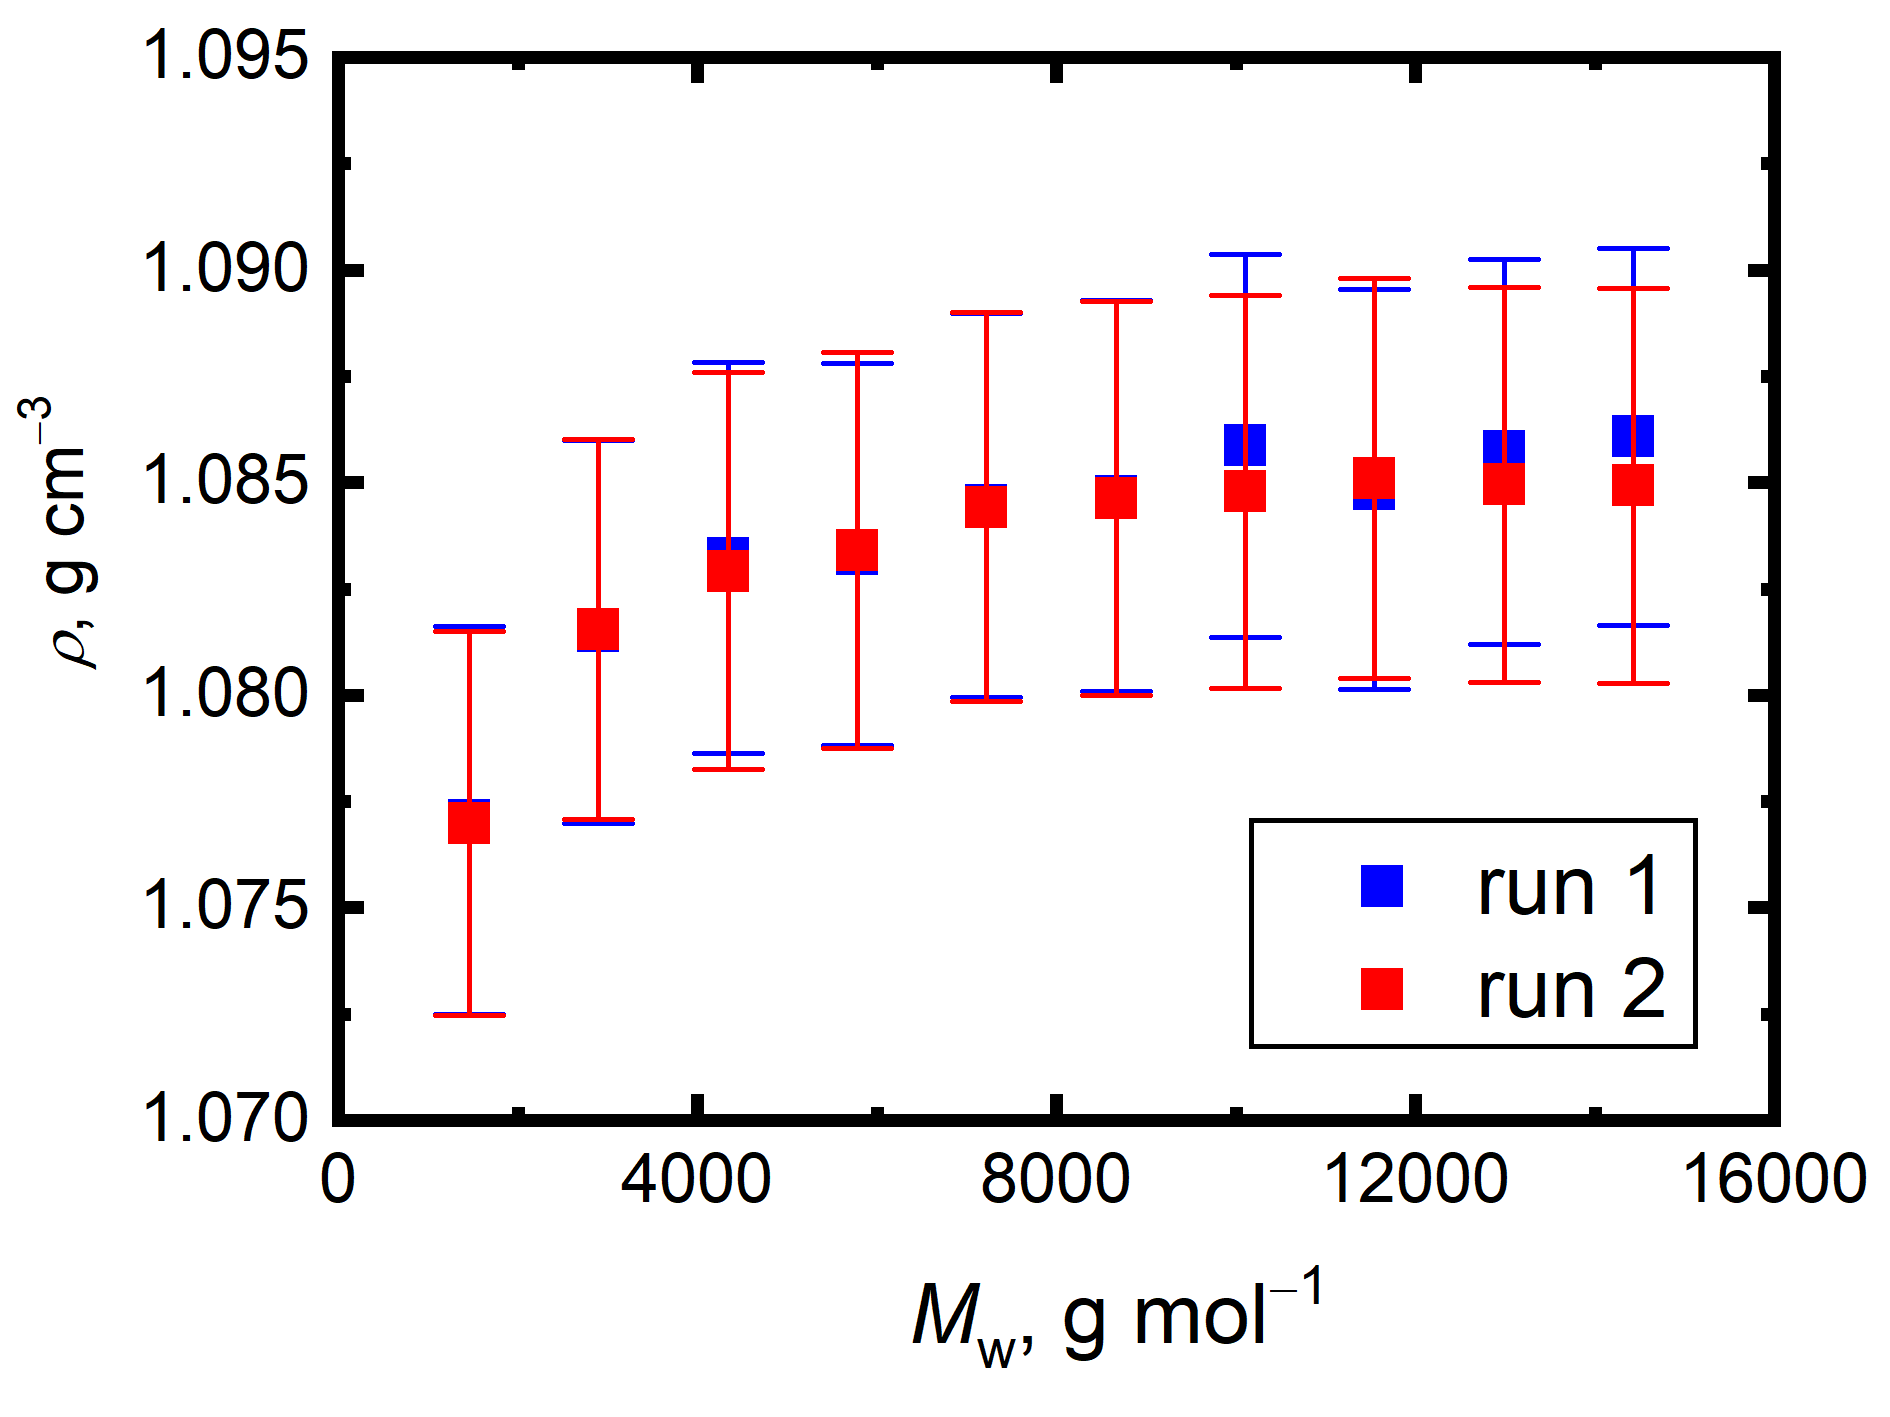
\includegraphics[width=1.0\linewidth]{img/pla_linear_density.png} 
		\caption{from initial fibrilar conformation}
		\vspace{-0.2cm}
	\end{subfigure}
	\begin{subfigure}{0.5\textwidth}
		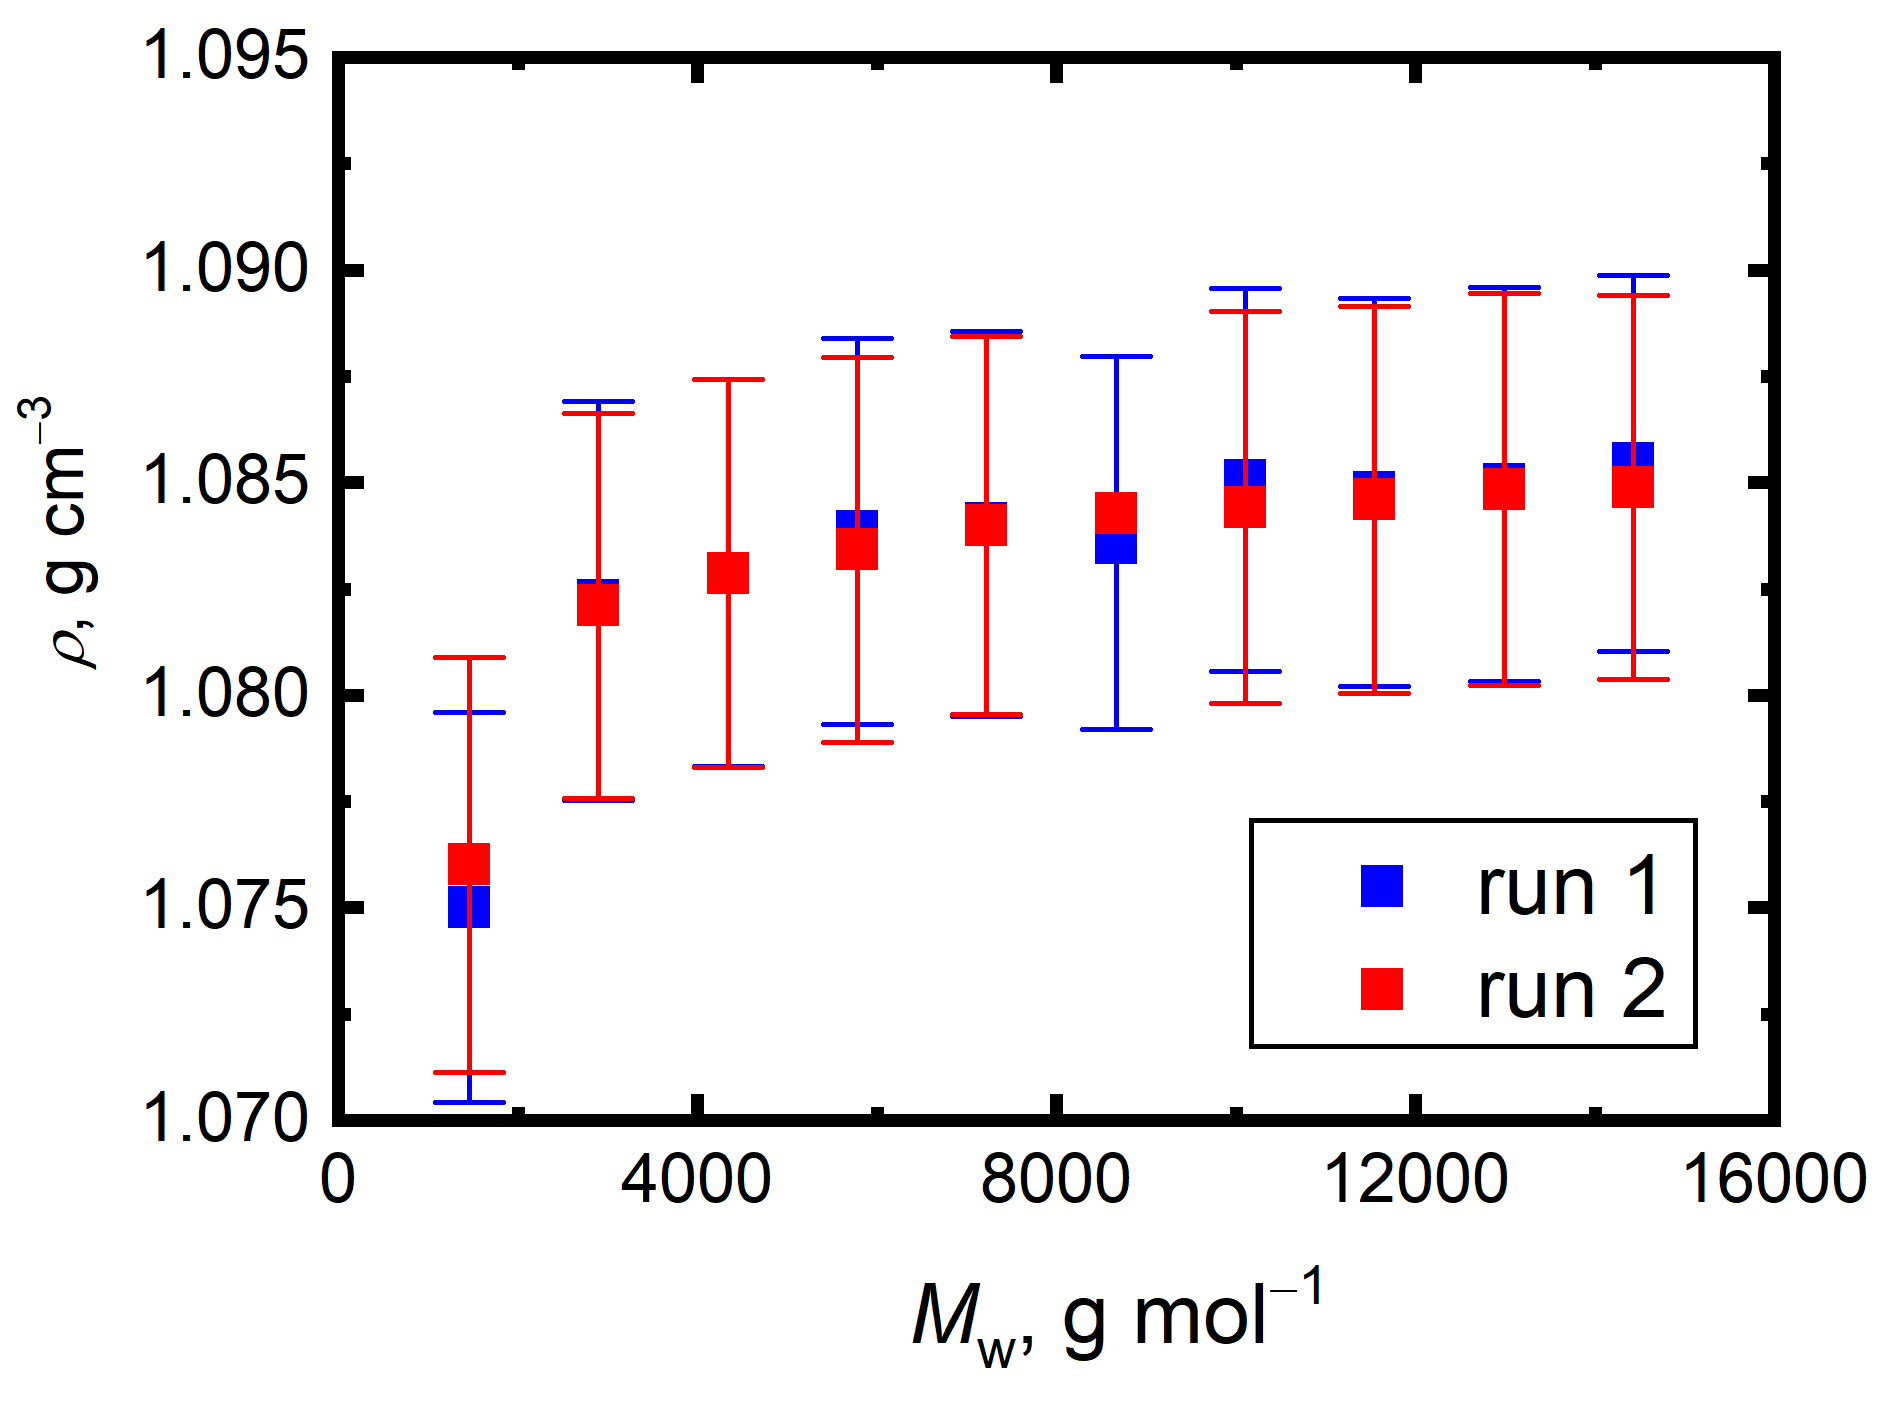
\includegraphics[width=1.0\linewidth]{img/pla_glob_density.png}
		\caption{from initial globular conformation}
		\vspace{-0.2cm}
	\end{subfigure} 
	\caption{Average densities with their standard deviations for PLA polymer chains at 500 K and 1 bar as a function of the chain length before (run 1) heating and (run 2) after cooling.}
	\label{fig:pla_hustoty}
	\vspace{-0.2cm}
\end{figure}

From the density data, any impact of the conformation memory cannot be assessed, since the bulk density is too a crude point of view on the polymer structure. That is the reason why the distances of the polymer chain termini that are displayed in the Figure \ref{fig:pla_konce} were calculated. The simulated time of 10 ns at the elevated temperature 1000 K was not enough to completely erase the polymer conformational memory, there is a noticeable deviation of the data sets obtained from the simulation initiated from the fibrilar and globular conformations.

\begin{figure}[htb!]
	\begin{subfigure}{0.5\textwidth}
		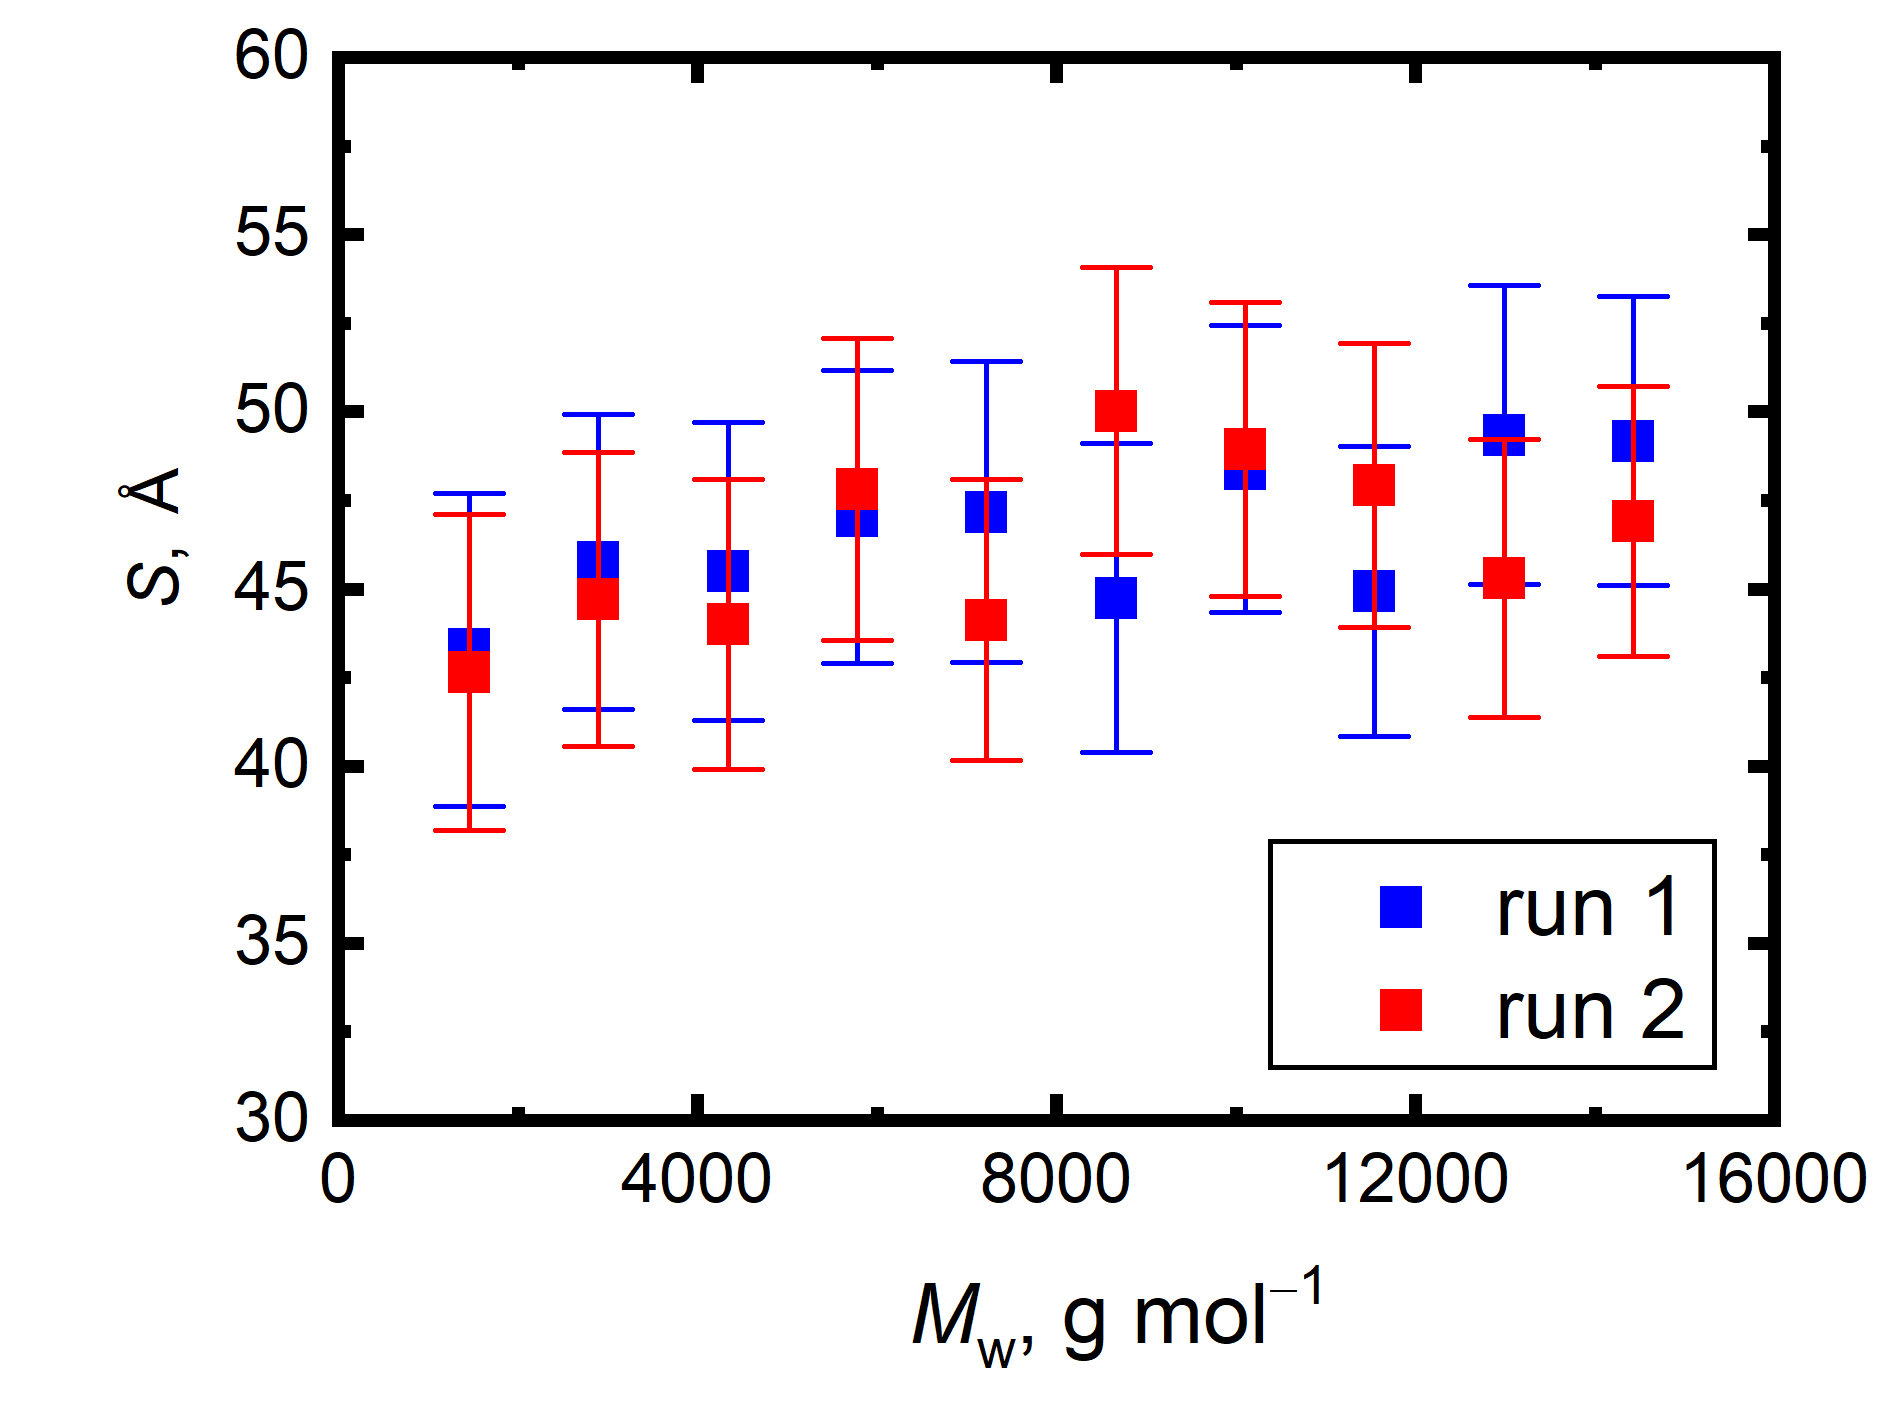
\includegraphics[width=1.0\linewidth]{img/pla_linear_konce.png} 
		\caption{from initial fibrilar conformation}
		\vspace{-0.2cm}
		\label{fig:subim1}
	\end{subfigure}
	\begin{subfigure}{0.5\textwidth}
		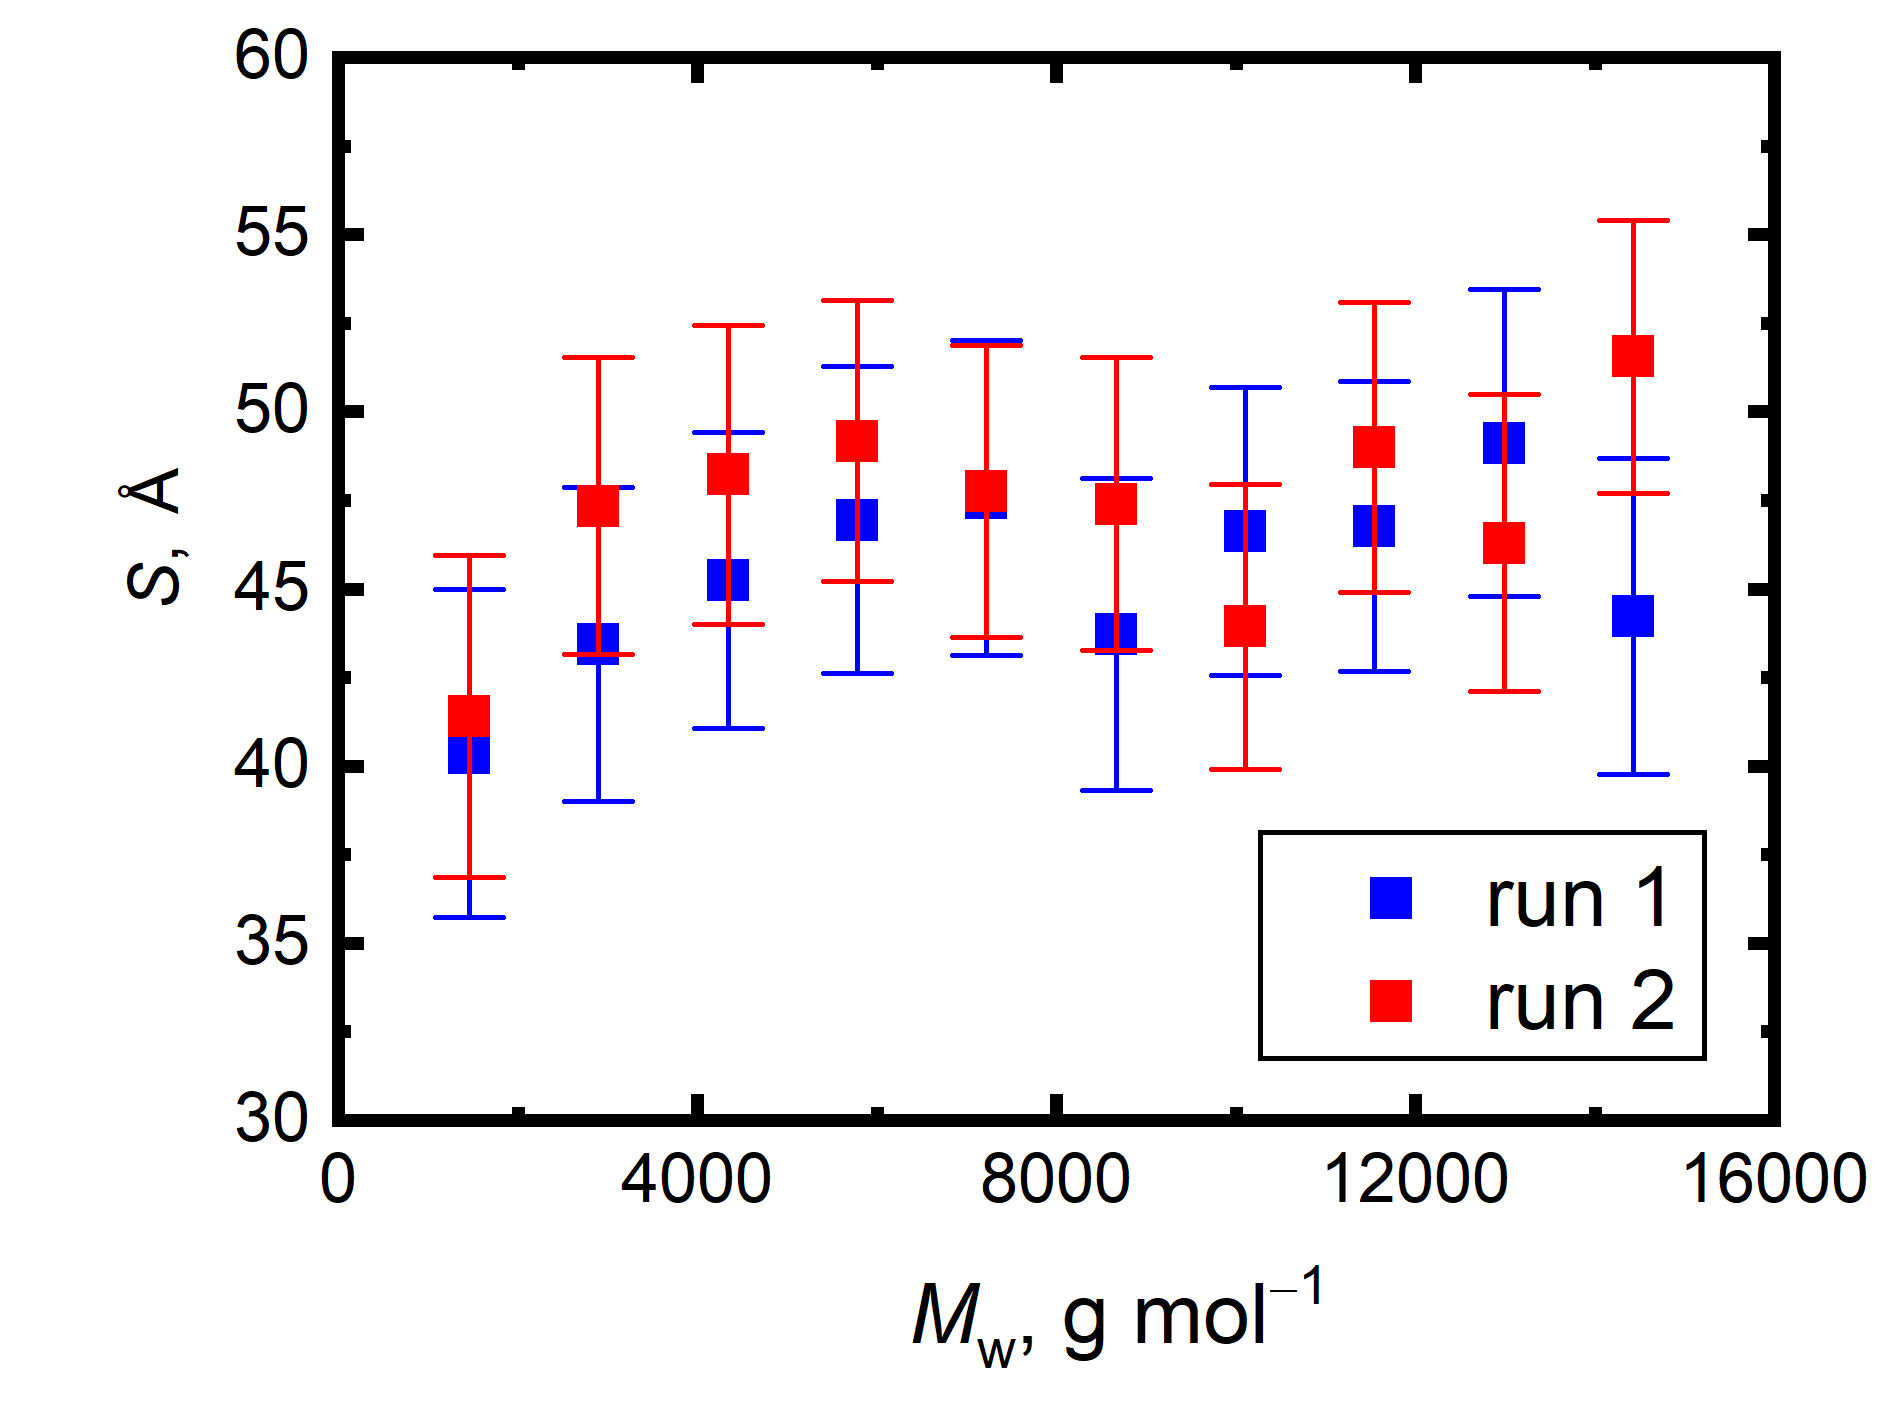
\includegraphics[width=1.0\linewidth]{img/pla_glob_konce.png}
		\caption{from initial globular conformation}
		\vspace{-0.2cm}
		\label{fig:subim2}
	\end{subfigure}
	\caption{Root mean square distances of the polymer chain termini with their standard deviations  for PLA polymer chains as a function of chain length before (run 1) heating and (run 2) after recooling.}
	\label{fig:pla_konce}
\end{figure}      

The dynamics of the polymer is slow due to complex entanglement of individual chains even at elevated temperatures, for a complete loss of the conformational memory it would be necessary to simulate the system for a longer period of time, especially for longer chains.

To investigate the effect of the box size on the molecular simulations, the simulations with boxes containing 5-50 polymer chains inside, each having a molar mass 12 989 $\mathrm{g \ mol^{-1}}$ were performed. The simulations were performed with a 3-block initial equilibration at 1000 K and 1 bar and subsequently cooled to 500 K and simulated for 10 ns. Mean densities obtained from these simulations are shown in the Figure \ref{fig:box} on the left. The simulation results prove that the size of the box has no significant effect on resulting average density. However, there is a visible effect of a lower uncertainty of standard deviations of densities for larger boxes. To have a better insight what is going on the structural level, we also analyzed the root-mean-squared end-to-end distance of the polymer chain termini shown in Figure \ref{fig:box_konce} on the right. From the obtained data, there is visible growing trend in end-to-end distances. That means that the small boxes are not sufficient to represent correctly the distribution of the end-to-end distances in the polymer. We can say, that its value converges for boxes containing more than 40 polymer chains. As a conclusion, when we are focused only on macroscopic properties such as density, we can use smaller number of chains in the simulation boxes in order to save the computational resources. However, when dealing with structural properties, we should be careful and set the number of chains in a simulation box more carefully.

\begin{figure}[htb!]
	\begin{subfigure}{0.5\textwidth}
		\centering
		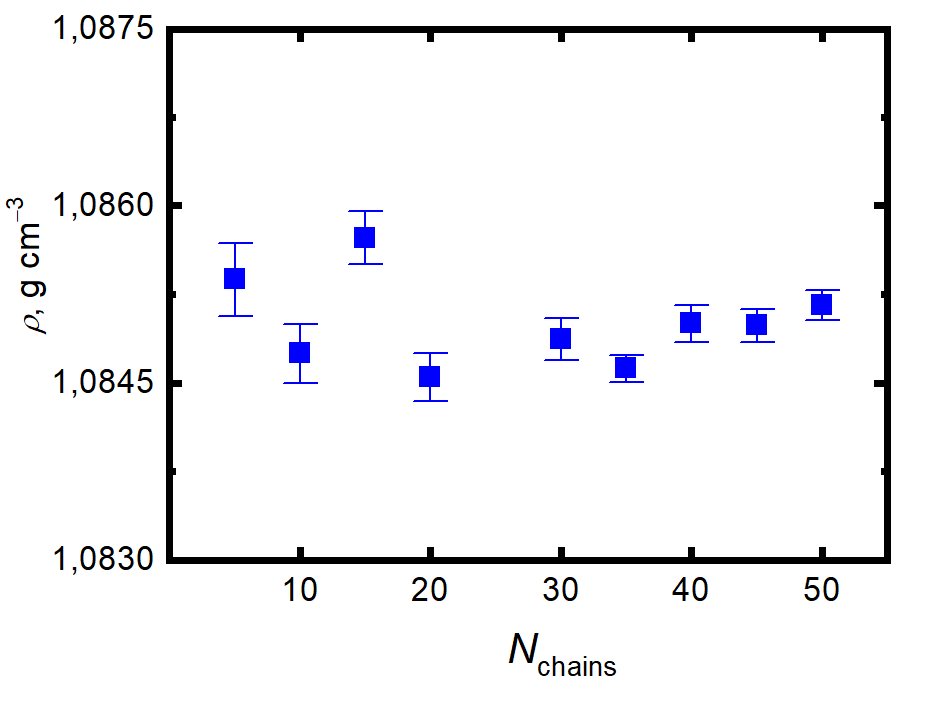
\includegraphics[width=1\linewidth]{img/hustota_5_50_sigma.png}
		\caption{}
		\label{fig:box}
	\end{subfigure}
	\begin{subfigure}{0.5\textwidth}
		\centering
		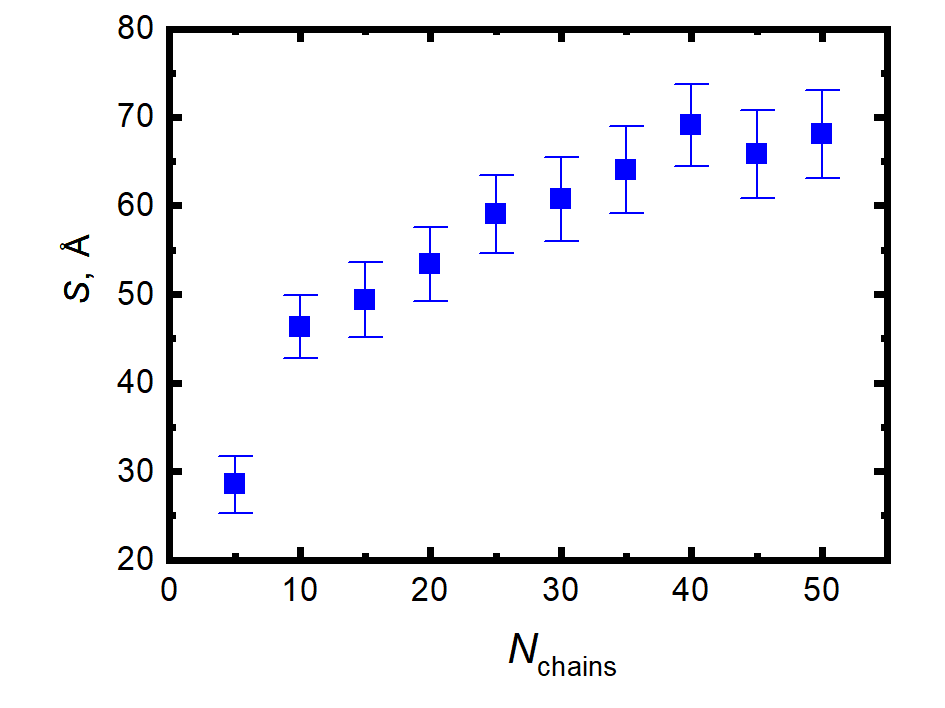
\includegraphics[width=1\linewidth]{img/konce_5_50.png}
		\caption{}
		\label{fig:box_konce}
	\end{subfigure}   	
	\caption{(a) dependence of density on the number of PLA polymer chains containing 90 dimer units in the box on the left and (b) dependence of root mean square distances of the polymer chain termini with their standard deviations on the right}
	\vspace{-0.2cm}
\end{figure}

To assess the accuracy of the calculated densities, the corresponding experimental data was obtained from literature. The comparison for two temperatures (300 and 500~K) in following Table \ref{tab:PLA_dens} was taken from \cite{klajmon_glass_2023}, where the methodology is also described in more details.

\begin{table}[htbp]
	\centering
	\caption{Comparison of calculated and experimental PLA denstities taken from \cite{klajmon_glass_2023}.}
	\begin{tabular}{cccc}
		\toprule
		$T$, K & $\rho_{\text{exp}},  \text{g cm}^{-3}$ & $\rho_{\text{MD}}, \text{g cm}^{-3}$ & $100(\rho_{\text{MD}}/\rho_{\text{exp}}-1)$\\
		\midrule
		 300   & $1.373 \pm 0.003$ & $1.193 \pm 0.001$ & $-13$\\
		 500   & $1.181 \pm 0.003$ & $1.086 \pm 0.001$ & $-8.0$ \\
		\bottomrule
	\end{tabular}%
	\label{tab:PLA_dens}%
\end{table}%

The experimental density value for 300 K is 13 \% above the computed, for 500~K the value is 8 \% above the computed density. In both cases, the value is higher than our limit value for the longest PLA polymer chain composed of 200 units.
 
\subsubsection{Polydispersity effect}
Under real conditions, it is hardly possible to experimentally prepare a monodisperse polymer containing only one selected chain length. For this reason, we simulated several polydisperse systems, each exhibiting a different distribution of molar masses of individual molecular chains, containing a total number of 50 chains. Their lengths come from an interval 8-244 units. Polydispersity index PDI~=~1 corresponds to 50 chains of length 124 units, the other values were calculated using the equation \ref{eq:PDI}. We than build composition of the other systems using the Gaussian distribution with the mean value of 124 units. By this procedure, we were able to obtain the PDI up to 1.3. To reach PDI 1.4 and 1.5, we had to increase the numbers of very short and long polymer chains present in the box to get the desired PDI. Designed compositions of systems based on PDI values are displayed in the Figure \ref{fig:polydisperzita_vyskyt}. The density was again evaluated from the simulations, in this case as a function of the PDI.

\begin{equation}
	\text{PDI} = \frac{\sum_{i} N_{i} \cdot \sum_{i} N_{i} M_{i}^2}{\left(\sum_{i} N_{i} M_{i}\right)^2}
	\label{eq:PDI}
\end{equation}


\begin{figure}[htb]
	\centering
	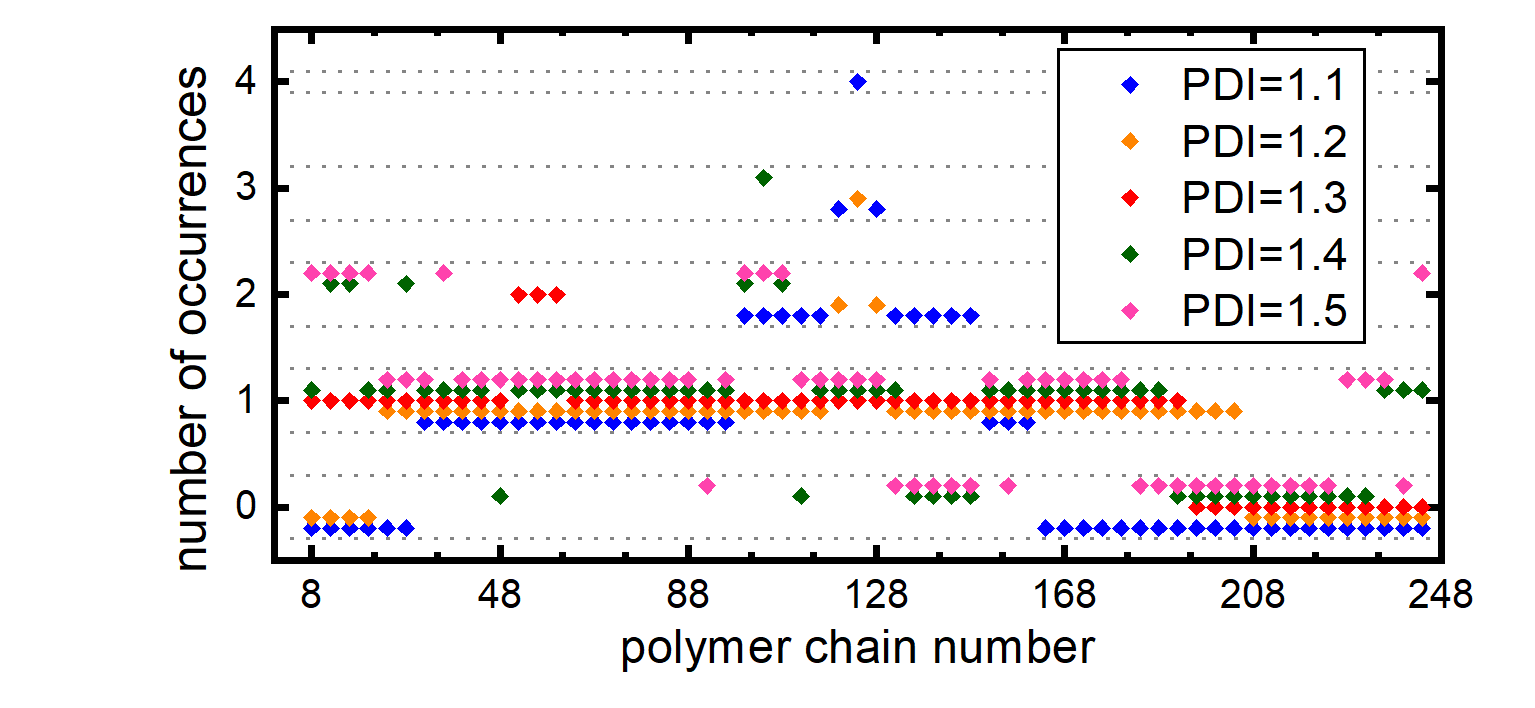
\includegraphics[width=1\hsize]{img/polydispersity_occurences_new.png}
	\caption{Number of occurrences of chains of a given length in the polydisperse systems with corresponding PDI.}
	\label{fig:polydisperzita_vyskyt}
\end{figure}       

Calculated densities depending on the PDIs are in the Figure \ref{fig:polydisperzita}. There is no significant difference among the densities obtained for different values of the polydispersity index. For the subsequent simulations we will use monodisperse systems as it will not introduce deviations from macroscopic behavior. 

\begin{figure}[htb]
	\centering
	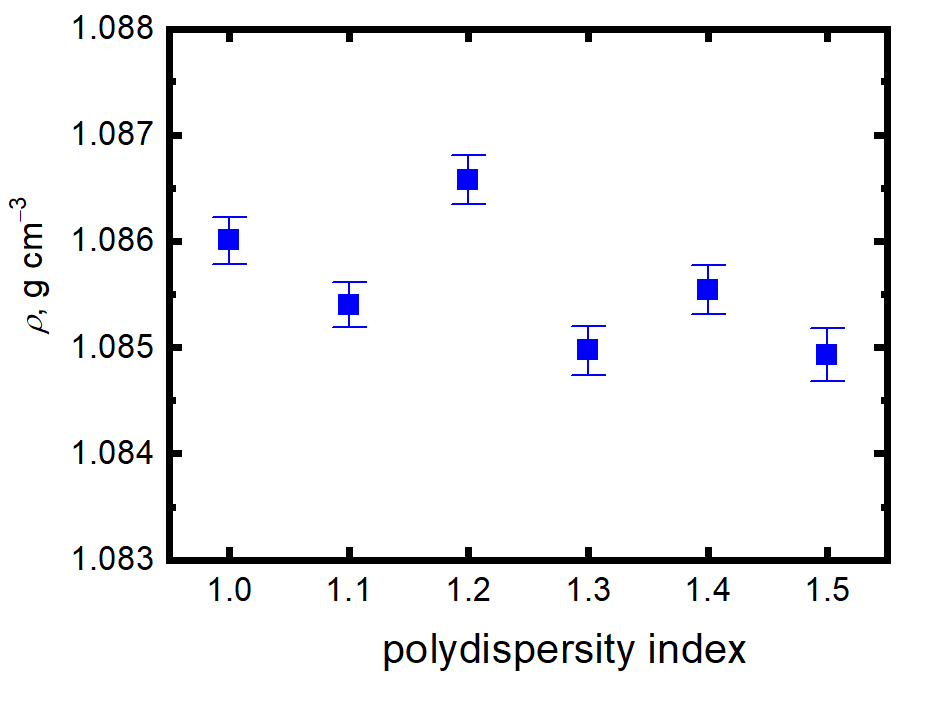
\includegraphics[width=0.5\hsize]{img/polydisperzita_new.png}
	\caption{Density of PLA at 500 K and 1 bar extracted from MD simulations depending on the polydispersity coefficients.}
	\label{fig:polydisperzita}
\end{figure}       

\subsubsection{Glass transition modeling}
Understanding the glass transition temperature of pharmaceutical materials is crucial for drug formulation, storage, and delivery. The $T_\text{g}$ refers to the temperature at which an amorphous material transitions from a rigid, glassy state to a more flexible, rubbery state without melting. The knowledge of $T_\text{g}$ helps us predict and control the stability of drugs during long-term storing.  

To obtain the glass transition temperature of PLA ($T_\mathrm{g}$), we started by simulating ten different polymer chain lengths for a set of temperatures in a range 140-485 K with a step of 15 K. For the system equilibration, each polymer chain simulation ran for 1 ns with a step of 1 fs. After the equilibration, the temperature interval for the following simulations was limited to the range of 200-485 K with a step of 15 K. Then, we run a $NpT$ production simulation for each temperature with this limited interval for 10 ns with a step of 1 fs from which the equilibrium bulk phase densities were calculated and displayed as a function of temperature. To get the glass transition temperature ($T_\mathrm{g}$) for PLA from volumetric data, the trend shift method was used \cite{klajmon_does_2022}. 

The trend shift method is illustrated for two different lengths of the polymer chains in the Figure \ref{fig:illust}. When we plot the bulk phase densities as a function of temperature, there is a visible trend shift which has the meaning of the transition between the glassy state and the rubbery state of a polymer. The point of the transition divides the density dataset into two intervals. Coordinates of the breakpoint and one surrounding point from each side were excluded from the further processing and the two resulting intervals were interpolated by a linear function. The $x$-coordinate of the intersection of these two lines determines the glass transition temperature. For this purpose a script in Maple software solving the system of linear equations was created to get the $T_\mathrm{g}$.

Available experimental $T_\mathrm{g}$ of L-PLA varies in the literature, the value  of $T_\mathrm{g}$ = 333 $\pm$ 4~K \cite{pyda_reversing_2005} was chosen as a reference value. The variation of experimental $T_\mathrm{g}$ data is caused by the stereo-configuration along the PLA chains, crystallinity of bulk PLA and the polydispersity. \cite{klajmon_glass_2023} The $T_\mathrm{g}$ value obtained in this work as an arithmetic mean of the values for all polymer chain lengths  is $T_\mathrm{g}$ = 337 $\pm$ 10~K. The calculated $T_\mathrm{g}$ for each polymer chain are displayed as function of polymer chain weight in the Figure \ref{fig:glass} with their arithmetic mean value drawn as a blue line. For each length of the polymer chain the regions for fitting were set manually. In the paper written by Klajmon et al\cite{klajmon_glass_2023}, the data value was obtained from the same data sets using automated script. Their resulted value is $T_\mathrm{g}$ = 351 $\pm$ 11~K. This corresponds with the fact that trend shift method is really sensitive to the intervals we determine, this is also illustrated in Figure \ref{fig:illust}. In this paper, there is also comparison with other methods used to determine in $T_\mathrm{g}$ and also with results for other polymers. 

The calculated $T_\mathrm{g}$ value is very close to the experimental one, there is no significant trend in $T_\mathrm{g}$ of polymer chain length of PLA from the calculated data. However, that small deviation between calculated and experimental value is more luck, when we compare the data for other polymers the difference is much larger.


\begin{figure}[H]
	\begin{subfigure}{0.5\textwidth}
		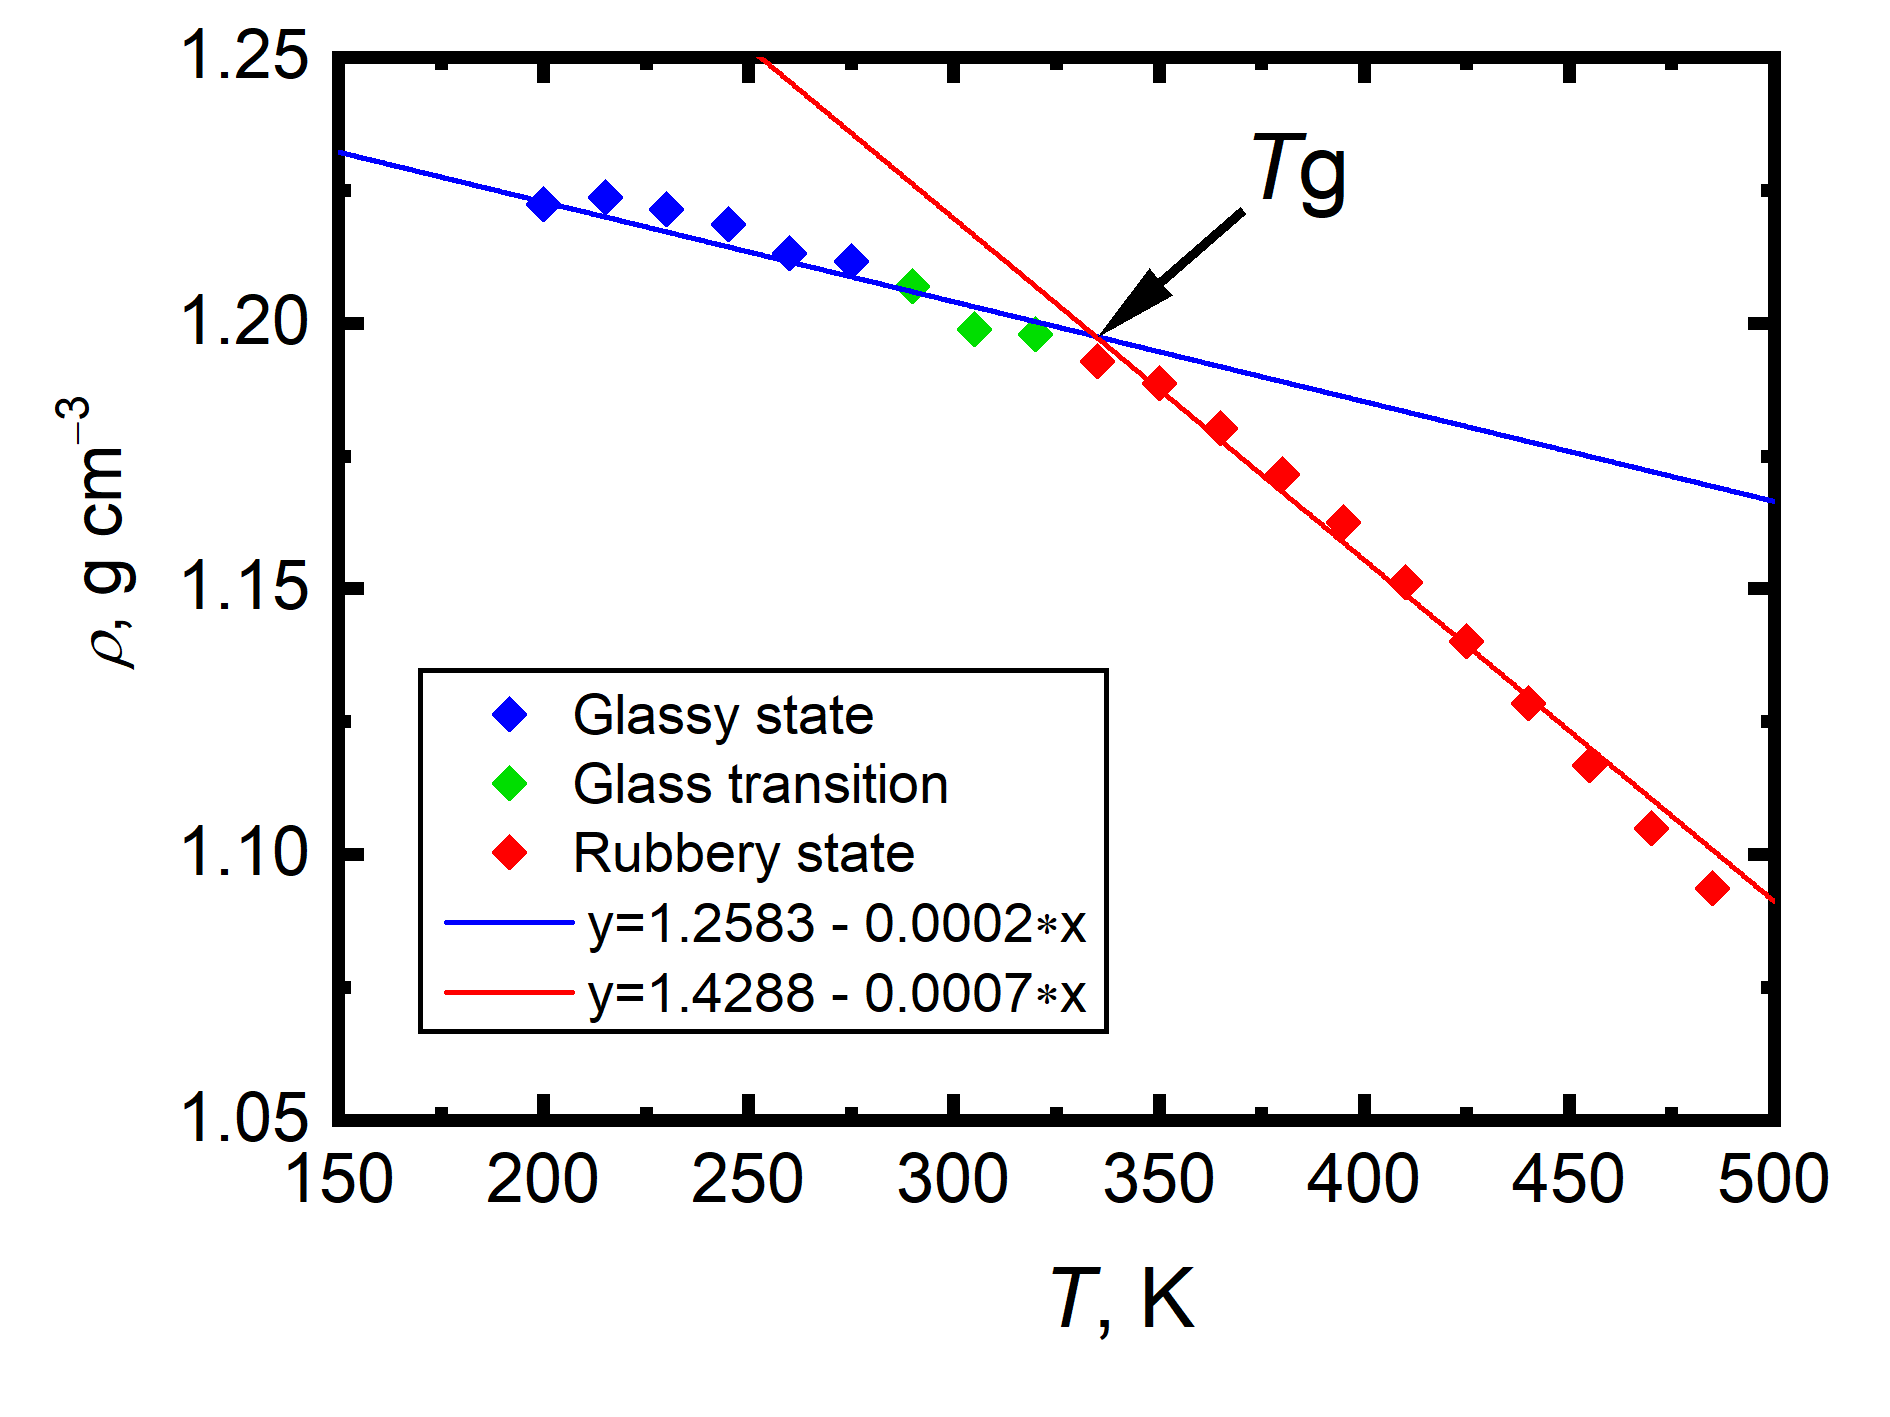
\includegraphics[width=1.0\linewidth]{img/vypocet_tg.png} 
	\end{subfigure}
	\begin{subfigure}{0.5\textwidth}
		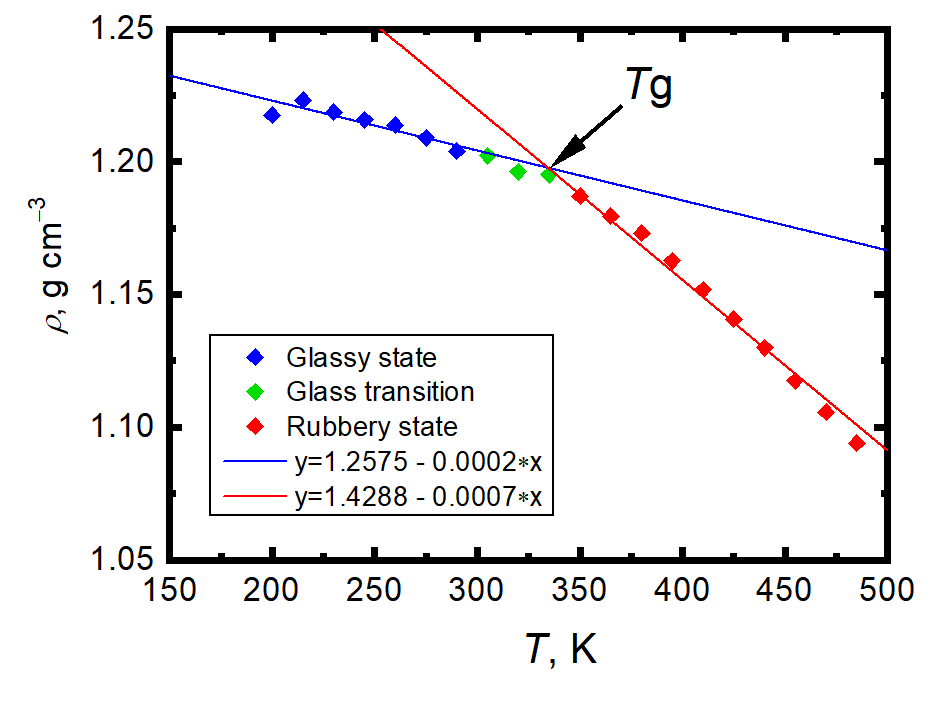
\includegraphics[width=1.0\linewidth]{img/tg_ukazka_30.png} 
	\end{subfigure}   	
	\vspace{-1cm}
	\caption{Illustration of the trend shift method for two polymer chains of different lengths, 20 units on the left and for 30 units on the right.}
	\label{fig:illust}
\end{figure}

\begin{figure}[htb!]
	\centering
	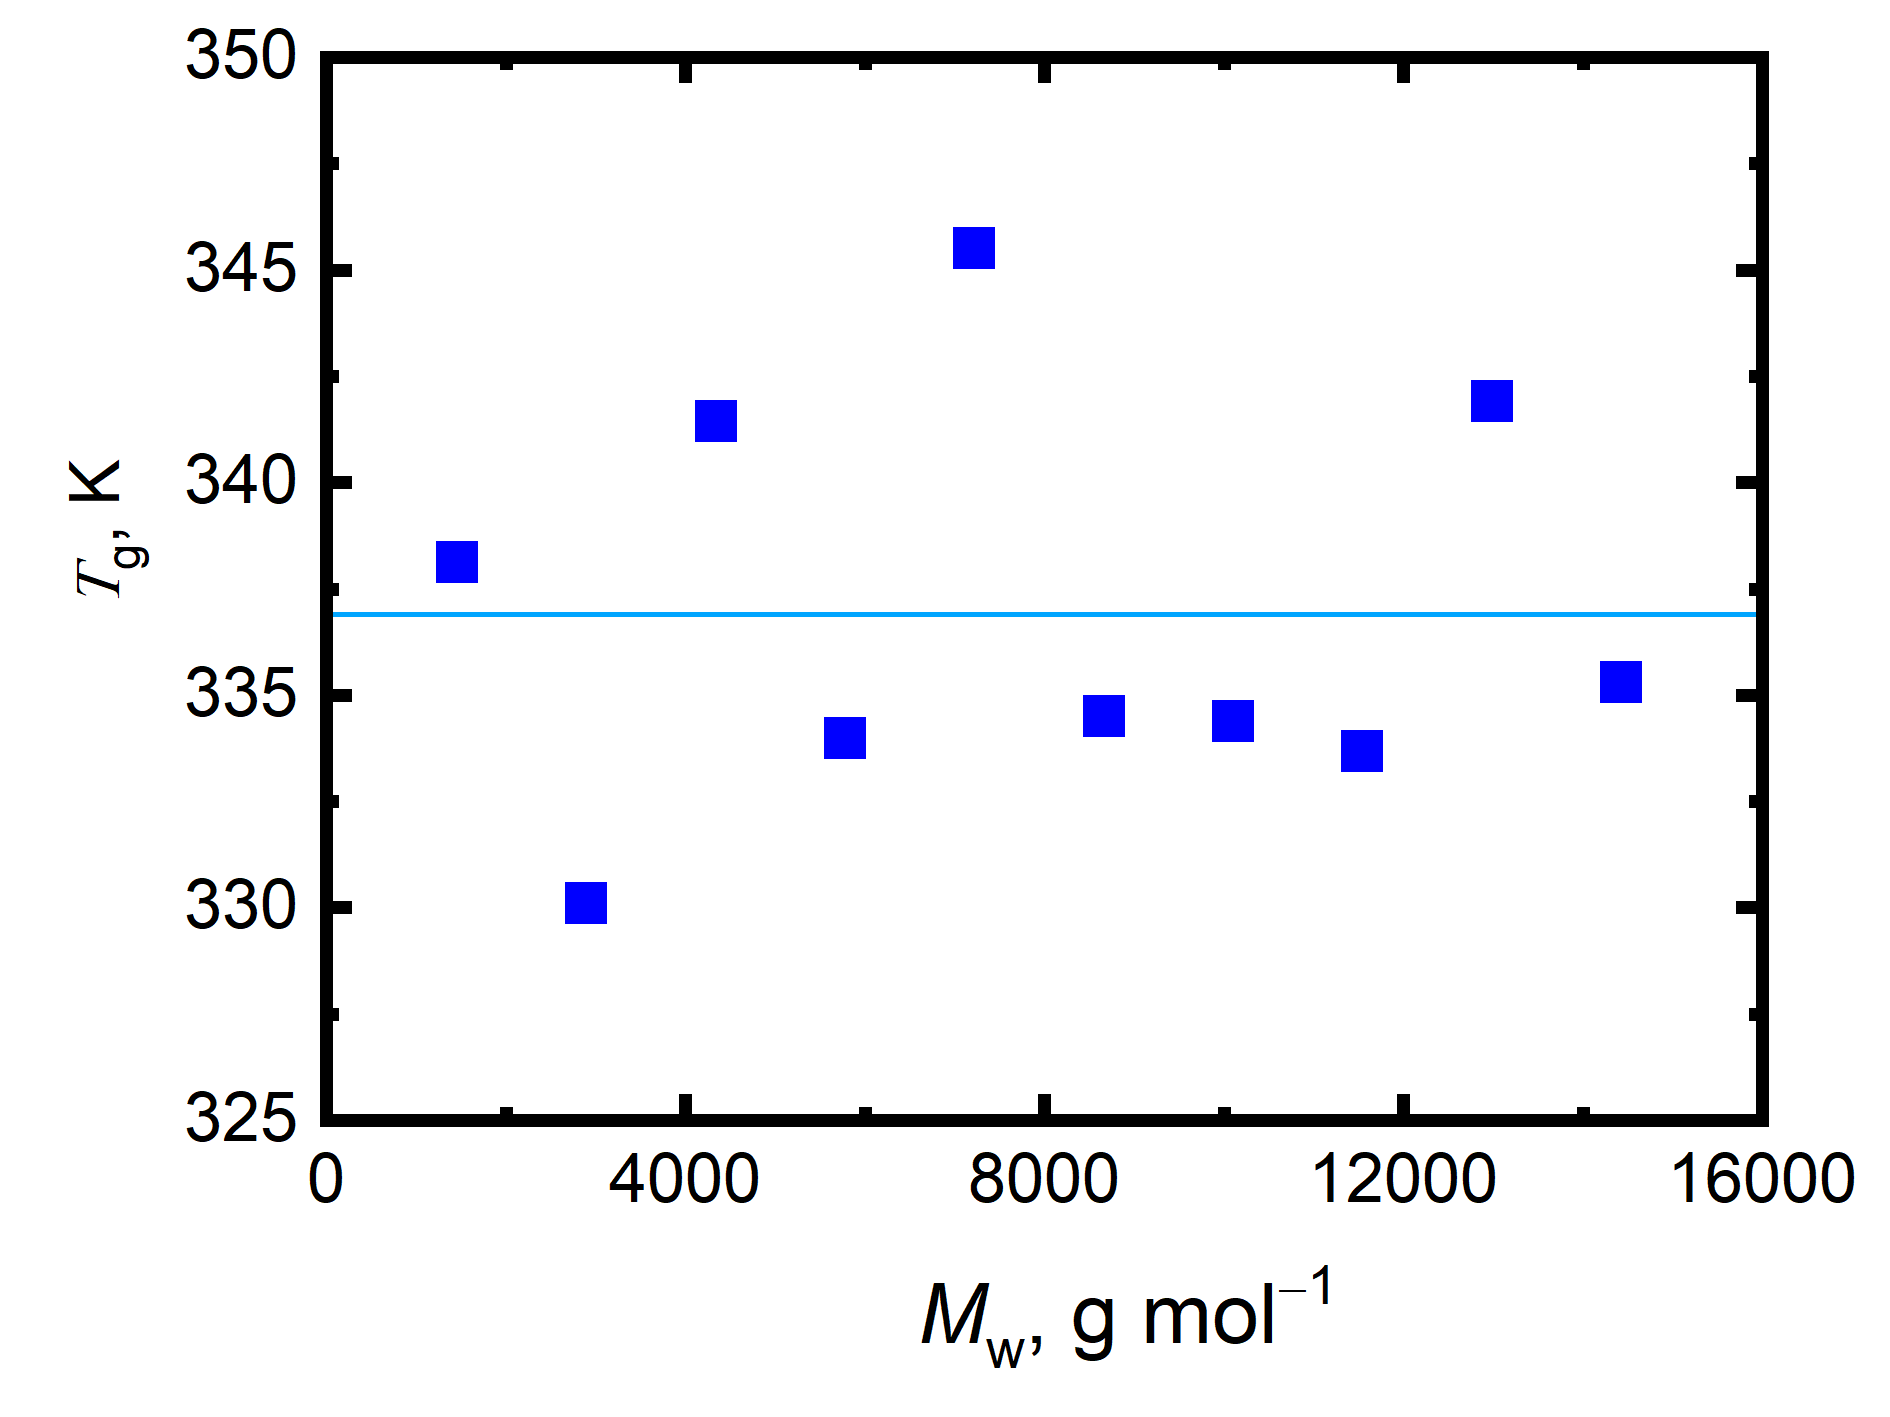
\includegraphics[width=0.5\linewidth]{img/glass_temp.png}
	\caption{Calculated $T_\mathrm{g}$ for all lengths of polymer chains using trend shift method, where blue line represents mean value.}
	\label{fig:glass}
\end{figure}

\newpage
\subsection{Simulations of neat API}
The parameters of API simulation boxes after the equilibration run ($T$=500 K) are presented in Table \ref{tab:API_n}, showing the number of API molecules ($N_{\text{API}}$), the total number of all atoms ($N_{\text{atoms}}$) and size of the cubic box ($l_{\text{box}}$).

\begin{table}[htb!]
	\caption{Properties of equlibrated simulations boxes for bulk API one-component systems, $T$=500 K.}
	\centering
	\begin{tabular}{lcccc} \toprule
		{\textbf{API}} & {\textbf{\boldmath{$N_{\text{API}}$}}} & \textbf{{\boldmath{$N_{\text{atoms}}$}}} & \textbf{{\boldmath{$M$, g mol$^{-1}$}}} & \textbf{{\boldmath{$l_{\text{box}}$, \AA}}} \\
			\midrule
			carbamazepine  & 800 & 24 000 & 236.27 & 66 \\		
			naproxen  & 800 & 24~800 & 230.26 & 66 \\
			ibuprofen  & 800 & 26~400 & 206.28 & 67 \\
			indomethacin  & 600 & 24~600 & 357.8 & 66 \\
			\bottomrule
		\end{tabular}
		\label{tab:API_n} 
	\end{table}
	
	To validate the force fields, computed densities were compared with experimental literature values, the comparison is in the Table taken from literature. UPRAVÍM \cite{cervinka_structure_2021}
	
	\begin{figure}[htb!]
		\centering
		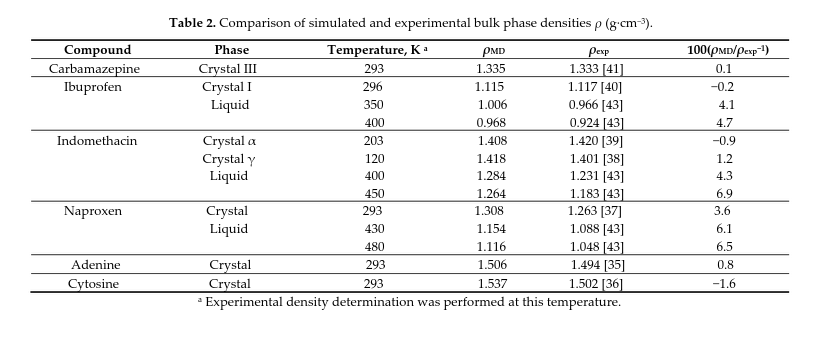
\includegraphics[width=1.0\linewidth]{img/tabulka_validace.png}
	\end{figure}

\subsubsection{Sulfathiazole FF parametrization}
A newly parametrized force field \cite{jorgensen_development_1996} was used for sulfathiazole. The charges on the atoms were calculated by quantum-chemical calculations using the Gaussian 16 code \cite{frisch_gaussian16_2016}. At first, the structure was optimized using the B3LYP functional with the aug-cc-pVTZ basis set with the dispersion correction GD3BJ \cite{smith_revised_2016}. After finding the optimal geometric structure of the molecule, the charges on the atoms were fitted through the CHELPG (Charges from ELectrostatic Potentials using a Grid-based method)\cite{breneman_determining_1990} method and inserted into force field file.
 
The MD simulations of the sulfathiazole crystal (polymorph II) were performed to validate the force field file parameters. The triclinic simulation box and barostat setting was used to account for the anisotropic character of the molecular crystal, other settings are similar to that with the PLA instead of calculating long-range interactions. The sulfathiazole crystal was simulated for three temperatures of 100, 200 and 300 K at 1 bar. The simulation results and experimental data obtained from literature \cite{drebushchak_crystal_2008} are given in the Table \ref{tab:sulfathiazol}. The MD simulations were performed with two different FF. First simulation was performed with FF field taken from literature (index MD1), second simulation with newly parametrized FF (CHELPG index). 
 
    \begin{table}[htb]   
    \caption{Comparison of simulated and experimental \cite{drebushchak_crystal_2008} crystallographic parameters for II polymorph of sulfathiazole. The index MD1 corresponds to force field taken from literature, index CHELPG to newly parametrized FF.}    
	\centering
	\begin{tabular}{lccc}
		\toprule
		$T$, K & 100 & 200 & 300\\
		\midrule
		$\rho_\mathrm{exp}$, g cm$^{-3}$  & $1.575(2)$ & $1.560(2)$ & $1.540(2)$\\
		$\rho_\mathrm{MD1}$, g cm$^{-3}$ & $1.552(1)$ & $1.534(2)$ & $1.515(2)$\\
		100($\rho_\mathrm{MD1}/\rho_\mathrm{exp}-1$) & $-1.5$ & $-1.7$ & $-1.6$\\
		$\rho_\mathrm{CHELPG}$, g cm$^{-3}$ & 1.525(1) & 1.538(2) & 1.495(2)  \\
		100($\rho_\mathrm{CHELPG}/\rho_\mathrm{exp}-1$) & $-3.2$ & $-1.4$ & $-2.9$\\
		\midrule
		$\beta_\mathrm{exp}$, $^{\circ}$ & $94.14(2)$ & $93.905(7)$ & $93.674(8)$\\
		$\beta_\mathrm{MD1}$, $^{\circ}$ & $91.56(7)$ & $91.6(1)$ & $91.7(1)$\\
		$\beta_\mathrm{CHELPG}$, $^{\circ}$ & 97.78(6) & 96.79(8) & 97.0(1)\\
		\midrule
		$a_\mathrm{exp}$, \AA & 8.1896(17) & 8.2122(7) & 8.2427(8)\\
		$a_\mathrm{MD1}$, \AA & 8.302(4) & 8.325(5) & 8.351(7) \\
		$a_\mathrm{CHELPG}$, \AA & 6.739(5) & 6.648(9) & 6.84(1) \\
		\midrule
		$b_\mathrm{exp}$, \AA & 8.532(2) & 8.5604(9) & 8.599(1) \\
		$b_\mathrm{MD1}$, \AA & 8.236(5) & 8.275(7) & 8.313(9) \\
		$b_\mathrm{CHELPG}$, \AA & 8.267(9) & 8.00(1) &	8.22(2) \\
		\midrule
		$c_\mathrm{exp}$, \AA  & 15.447(4) & 15.497(2) & 15.563(2) \\
		$c_\mathrm{MD1}$, \AA & 15.99(1) & 16.06(2) & 16.13(2) \\
		$c_\mathrm{CHELPG}$, \AA & 20.15(2) & 20.88(3) & 20.35(5)\\
		\bottomrule
	\end{tabular}
	\label{tab:sulfathiazol}
\end{table}

There is good agreement between the experimental and computed densities, the relative deviations low for both FF. Other parameters differs more between the two FF used. Generally, the MD1 FF describes better the $\beta$ angle and the parameters of the unit cell within all simulated temperatures. It would be also useful to obtain the data for liquid state and compare them with experiments.

\subsection{Simulations of mixtures of APIs and PLA}
The simulations of mixtures of 4 APIs with PLA were performed following the scheme described in previous methodology section 3.2. The images of the simulation boxes for mixtures with the least considered amount of API ($x_{\text{API}}=0.85$) for temperature 500~K are in figure \ref{fig:mix_boxes}. The polymer was represented by quicksurf drawing method and diffused in the background, the API molecules are represented with balls and sticks above the PLA molecules.

\begin{figure}[htb!]
	\centering
	\subfloat{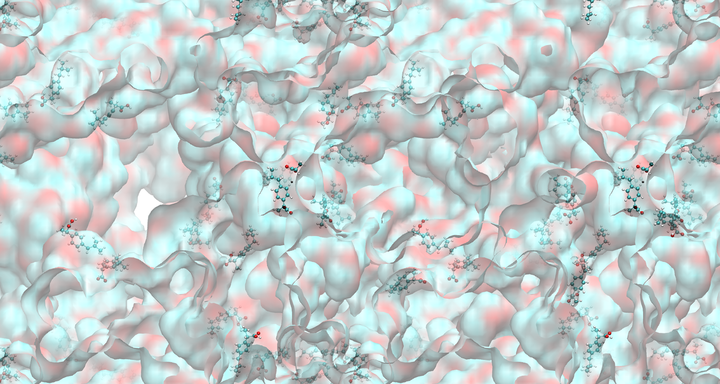
\includegraphics[width=0.47\linewidth]{img/ibu_s_100x_bp.png}}
	\hspace{0.2cm}
	\subfloat{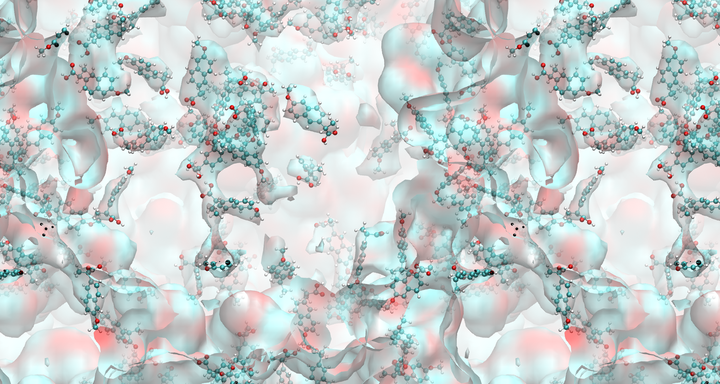
\includegraphics[width=0.47\linewidth]{img/nap_100x_bp.png}}\\
	\vspace{0.2cm}
	\subfloat{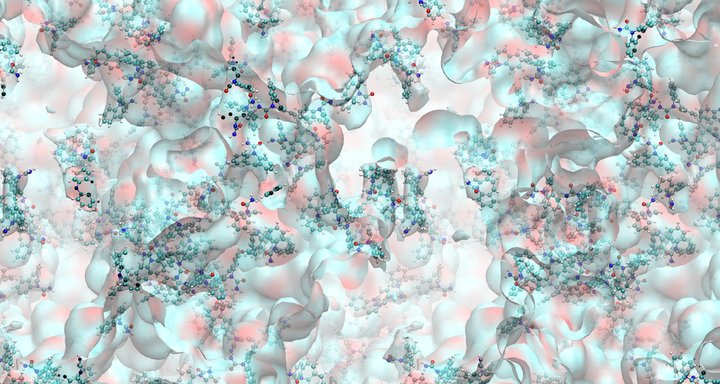
\includegraphics[width=0.47\linewidth]{img/cbz_100x_bp.png}}
	\hspace{0.2cm}
	\subfloat{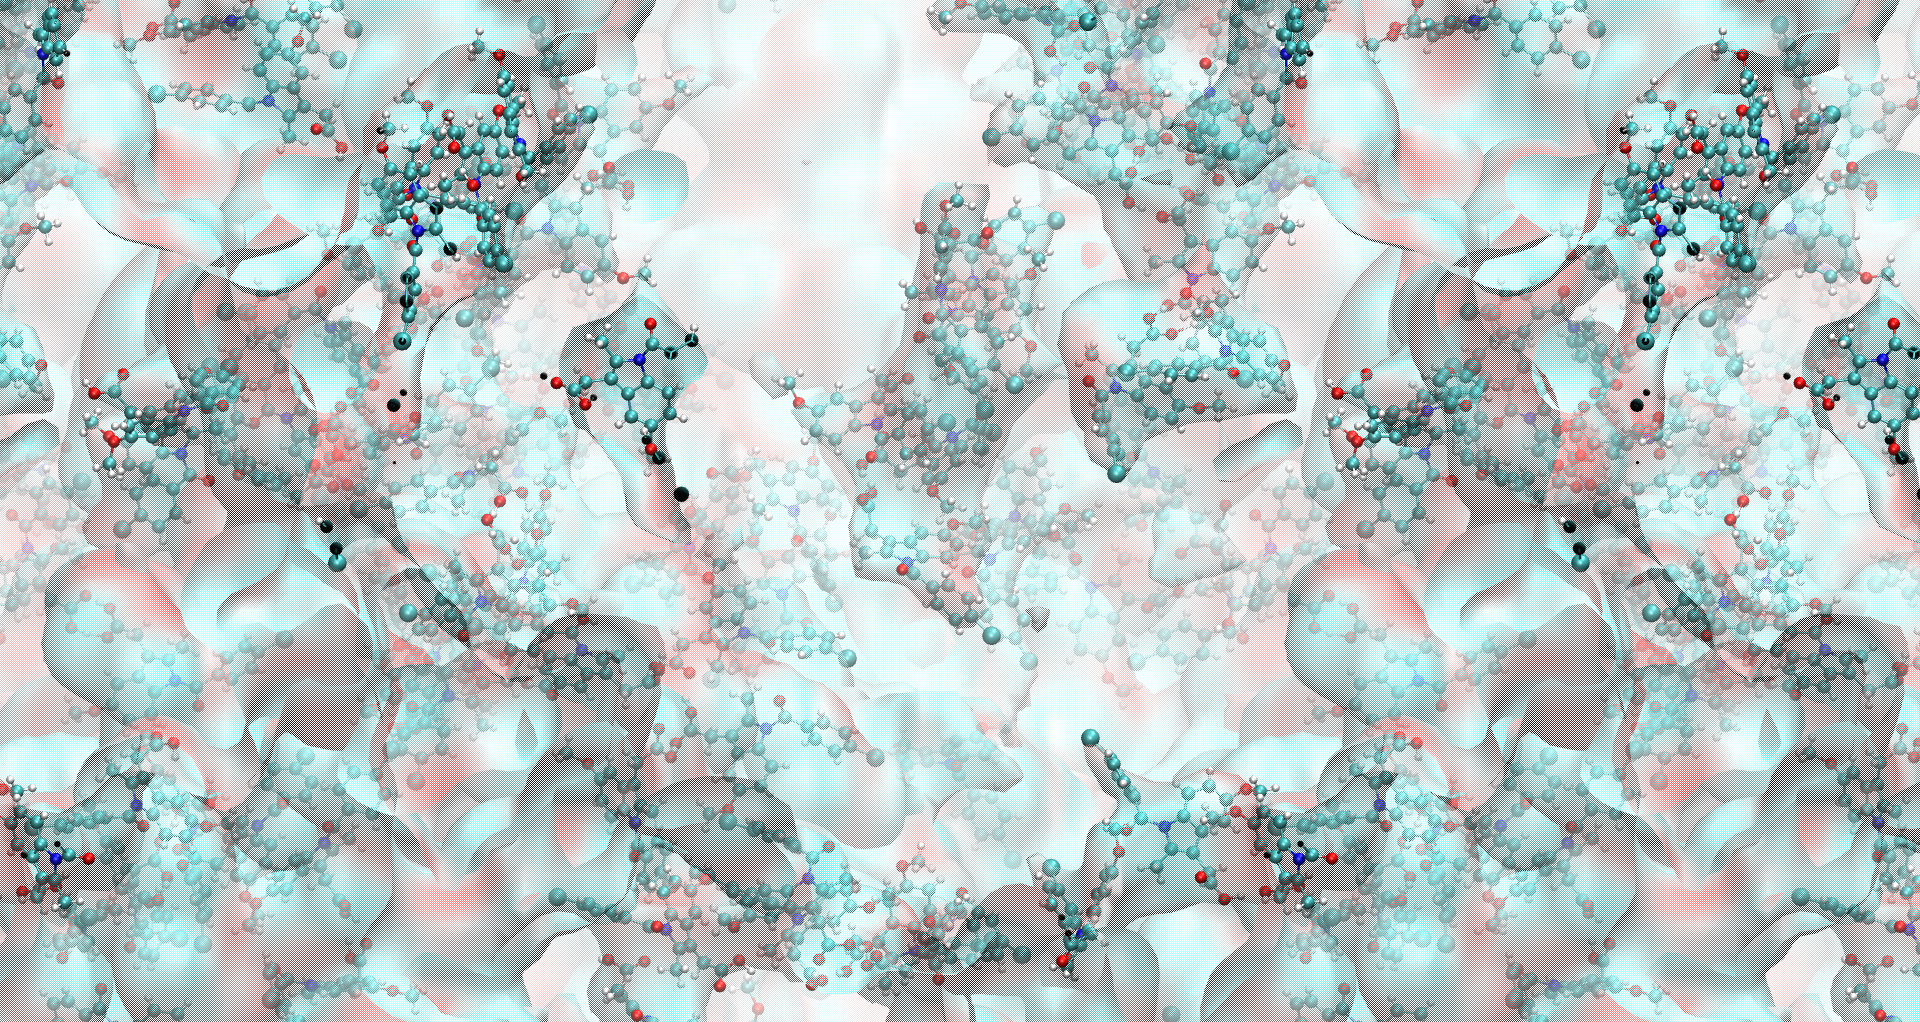
\includegraphics[width=0.47\linewidth]{img/indo_100x_bp.png}}
	\caption{Image of the simulation box for $x_{\text{API}}=0.85$ and $T=500~K$ for ibuprofen (\textbf{top left}), naproxen (\textbf{top right}), carbamazepine (\textbf{bottom left}) and indomethacin (\textbf{bottom right}).}
	\label{fig:mix_boxes}
\end{figure}
\vspace{-0.5cm}
\subsubsection{Excess properties}
Excess molar energy and excess molar volume are thermodynamic quantities that quantify deviations from ideal behavior in solutions. Ideal solutions exhibit symmetry interactions between all components, resulting in linear relationships between the properties of the mixture and its composition. However, real solutions often deviate from the ideal behavior due to the asymmetry interactions between molecules such as hydrogen bonding or their steric disproportions.

The excess molar energy represents the additional energy per a mole of mixture compared to an ideal solution at the same temperature, pressure, and composition. It accounts for the energy associated with interactions between molecules in the mixture, including both attractive and repulsive forces. Negative excess molar energies indicate favorable interactions (in our case mostly hydrogen bonding), while positive values suggest repulsive interactions. Excess molar energies of the mixtures were evaluated by the Equation \ref{eq:EM}

%\vspace{-0.1cm}
\begin{equation}\label{eq:EM}
	E^\text{E} = E_{\text{m}}^{\text{MIX}} - x_{\text{API}} E_{\text{m}}^{\text{API}} - x_{\text{PLA}} E_{\text{m}}^{\text{PLA}},
\end{equation}

where $E_{\text{m}}^{\text{MIX}}$ is the average molar energy of the simulation box of the mixture, $E_{\text{m}}^{\text{API}}$ is the average molar energy of pure API, and $E_{\text{m}}^{\text{PLA}}$ is the averaged molar energy of pure PLA obtained from simulations. 

Similarly, the excess molar volume quantifies the deviation in the volume per a mole of a mixture from that of an ideal solution. It reflects the changes in volume resulting from interactions between molecules, such as volume contraction due to strong molecular association or volume expansion due to repulsive interactions.

Excess molar volumes ($V^{\text{E}})$ of the mixtures were evaluated from the simulations for each concentration using the Equation \ref{eq:VM}. For this reason, the average molar volumes of the simulation boxes were evaluated from simulations of pure API ($V_{\text{m}}^{\text{API}} $) and pure polymer ($V_{\text{m}}^{\text{PLA}}$) and from a mixture ($V_{\text{m}}^{\text{MIX}}$) of API and PLA. To obtain the uncertainties block averaging scheme and error propagation law was used. 
 
%\vspace{-0.2cm}

\begin{equation}\label{eq:VM}
	V^{\text{E}} = V_{\text{m}}^{\text{MIX}} - x_{\text{API}} V_{\text{m}}^{\text{API}} - x_{\text{PLA}} V_{\text{m}}^{\text{PLA}}
\end{equation}

Mixing energies and volumes were calculated for all systems and both temperatures (300, 500~K), and the comparison is shown in Table \ref{tab:vobjemy}.  
%\vspace{-0.2cm}



\begin{table}[htb]
	\caption{Calculated excess energies (kJ mol$^{-1}$) and volumes (in cm$^3$ mol$^{-1}$) for API mixtures of different concentrations from simulations under 300~K ($V_{300}^\text{E}$, $E_{300}^\text{E}$) and 500~K ($V_{500}^\text{E}$, $E_{500}^\text{E}$) with their standard uncertainties (k=1).}
	\vspace{-0.2cm}
	\centering
	\begin{tabular}{lSSSSSSSSS}
	\toprule
	\textbf{API} & \boldmath{$x_{\text{API}}$} & \boldmath{$V_{300}^\textbf{E}$} & \boldmath{$\sigma_{V^\textbf{E}}$} & \boldmath{$V_{500}^\textbf{E}$} & \boldmath{$\sigma_{V^\textbf{E}}$} & \boldmath{$E_{300}^\textbf{E}$} & \boldmath{$\sigma_{E^\textbf{E}}$} & \boldmath{$E_{500}^\textbf{E}$} & \boldmath{$\sigma_{E^\textbf{E}}$} \\
	\midrule
		\text{cbz} & 0.85 & -5.47 & 0.27 & 0.92 & 0.50 & 0.63 & 0.30 & 4.74 & 0.46 \\
		& 0.92 & -3.45 & 0.14 & 0.64 & 0.27 & 0.54 & 0.15 & 3.20 & 0.21 \\
		& 0.95 & -2.34 & 0.11 & 0.22 & 0.17 & -0.09 & 0.11 & 2.65 & 0.16 \\
		\midrule
		\text{nap} & 0.85 & -5.04 & 0.27 & 3.28 & 0.48 & 4.38 & 0.24 & 7.49 & 0.44 \\
		& 0.92 & -2.16 & 0.16 & 2.61 & 0.26 & 3.88 & 0.24 & 6.26 & 0.26 \\
		& 0.95 & -1.81 & 0.10 & 1.46 & 0.18 & 3.39 & 0.10 & 4.72 & 0.20 \\
		\midrule
		\text{indo} & 0.85 & -7.33 & 0.26 & -1.24 & 0.54 & 5.20 & 0.25 & 8.55 & 0.65 \\
		& 0.92 & -3.85 & 0.13 & -1.73 & 0.28 & 4.70 & 0.16 & 6.37 & 0.29 \\
		& 0.95 & -2.96 & 0.17 & -2.00 & 0.22 & 2.04 & 0.15 & 3.53 & 0.31 \\
		\midrule
		\text{ibu} & 0.85 & -9.63 & 0.33 & 0.25 & 0.49 & -1.27 & 0.35 & 3.28 & 0.42 \\
		& 0.92 & -6.45 & 0.21 & 0.11 & 0.29 & -0.34 & 0.17 & 2.63 & 0.24 \\
		& 0.95 & -5.29 & 0.12 & -0.14 & 0.17 & 0.23 & 0.16 & 2.12 & 0.15 \\
	\bottomrule
	\end{tabular}
	\label{tab:vobjemy} 
\end{table}
\vspace{-0.2cm}
For the lower temperature of 300~K, all excess volumes ($V^\text{E}$) are negative, indicating a more beneficial spacial packing. The lowest value is for indomethacin, which indicates better spatial configuration. Indomethacin also exhibited the strongest interactions corresponding to the highest RDF first peak among other API. For all APIs, there is visible trend, with higher concentration of PLA the $V^\text{E}$ value is lower. The same trend is observed for excess energies for 3 of 4 APIs (CBZ, NAP, INDO), for ibuprofen the trend of $E^\text{E}$ is the opposite. 

For the higher temperature of 500~K, all excess energies are positive, this indicate that addition of the polymer can attenuate the API-API interactions, but those are not fully compensated by creating new intermolecular interactions between API and PLA in the mixtures. We can see, that for higher concentration of API in the mixture ($x_{\text{API}}$) the values of $E^\text{E}$ are decreasing also with their uncertainties. The reason could be that more interactions of API-API are still presented resulting in less frequent API-PLA interactions that do not exhibit the potential to compensate the API-API cohesion. The analysis of radial distribution functions of the most favorable interactions between API-API and API-PLA was performed in order to see the which specific interactions are forming. Same trend was observed for the height of the first peak for different concentrations. Complete results are given in following section.

The excess volumes are also decreasing with higher concentration of API in the mixture. For carbamazepine and naproxen, the $V^\text{E}$ values are already positive at 300~K, meaning less advantageous packing of molecules in space. For indomethacine, all values are negative, a sterically more advantageous arrangement is thus observed for its mixtures. For ibuprofen, the values are close to zero, for the highest API concentration the value is negative. This indicate minimal sterical effect of mixing. 



\vspace{-0.1cm}

\subsubsection{Radial distribution functions}
\vspace{-0.2cm}
Sampling the radial distribution functions from the simulations was done to explore the interactions that are having the highest impact on the material cohesion. The hydrogen bonds were mostly studied as the most important cohesive features. First, the important homomolecular API-API contacts are discussed, then API-PLA interactions are studied.



\newpage
\textbf{API-API interactions}
The strongest API-API interaction was identified with respect to RDF amplitudes and plotted to study the change between neat API and simulations of mixtures with different concentrations of PLA. For ibuprofen, naproxen and indomethacine, the interaction between the oxygen and hydrogen atoms from carboxyl group was studied. However, carbamazepine does not contain a complete carboxyl group, the hydrogen bonding was studied between the N$\text{H}_\text{2}$ and OC group. The selected atom types involved in respective molecular interactions are visualised in the introduction section in Figure \ref{fig:APIs}. 

The LAMMPS MD simulation software is normalizing the RDF signal to the density of the system, meaning that different RDF values are corresponding to systems with neat API and mixtures. Due to that reason all RDFs of mixtures containing the API-API interaction were scaled onto the pure API RDF signal, enabling us to perform a direct comparison of the amplitudes of individual signals. The following Equation \ref{eq:RDF_formula} was used.\vspace{-0.5cm}

\begin{equation}\label{eq:RDF_formula}
	\text{RDF}_{\text{scaled}} = \text{RDF} \cdot \frac{V_{\text{API}}}{N_{\text{API}}} \frac{N_{\text{mix}}}{V_{\text{mix}}},
\end{equation}

\vspace{-0.2cm}

where $V_{\text{API}}$ is the average volume of the pure API simulation box, $N_{\text{API}}$ is the number of molecules in the pure API simulation box and analogously for mixtures.

The RDF of the hydrogen bonding interaction in between carboxyl group of indomethacin is shown in Figure \ref{fig:indo_RDF_}. The contact distance of the closest COOH dimer corresponding to the first peak is only 1.5 \AA for all concentrations. Indomethacin is forming very strong hydrogen bonded dimer contact in between carboxyl groups, the strongest in comparison to other studied APIs having COOH group. The first peak amplitude is extremely strong and decrease with less API in the mixture. There are also presented other O-H$\cdots$O contacts from neighboring carboxyl groups (second and third peak) at longer distances with much lower amplitudes. When the system is heated up to 500~K, there is less significant difference in amplitudes of peaks corresponding to different concentrations, also the interactions are having lower amplitudes. However, the first coordination sphere still contains one molecule, corresponding to the closest COOH dimer contact still saturated by its hydrogen bonds.

\begin{figure}[htb!]
	\centering
	\subfloat{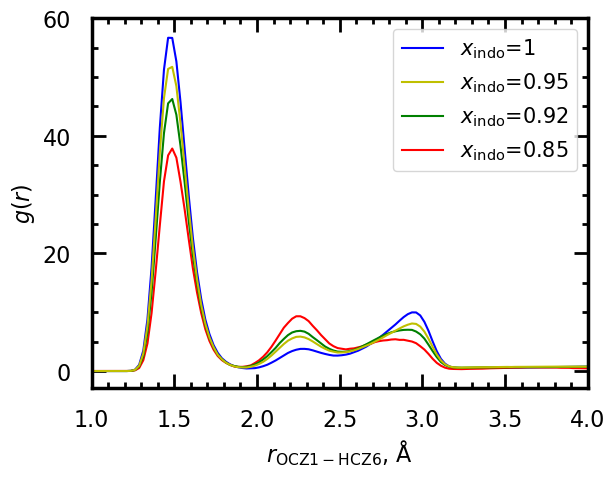
\includegraphics[width=0.4\linewidth]{img/rdf_indo_api_r3.png}}
	\subfloat{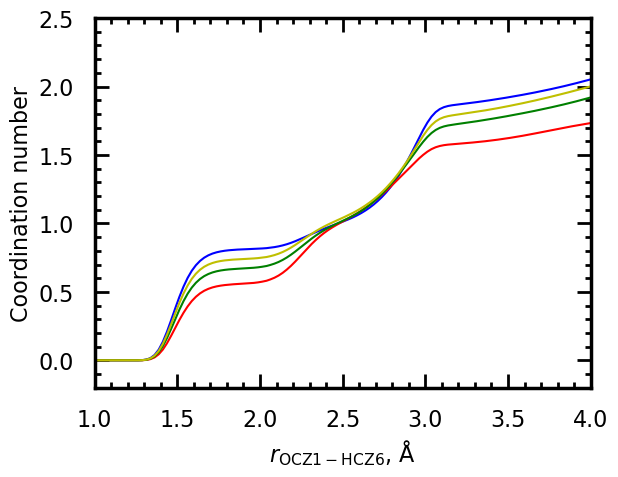
\includegraphics[width=0.4\linewidth]{img/coord_indo_api_r3.png}}\\
	\subfloat{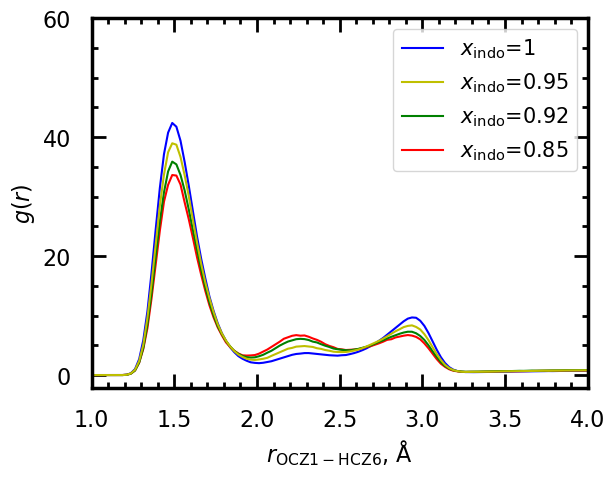
\includegraphics[width=0.4\linewidth]{img/rdf_indo_api_r2.png}}
	\subfloat{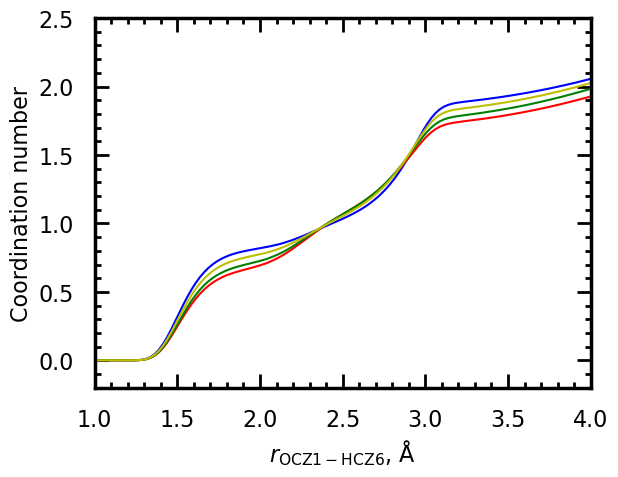
\includegraphics[width=0.4\linewidth]{img/coord_indo_api_r2.png}}
	\vspace{-0.3cm}
	\caption{RDF of the API-API interaction between HCZ6 hydrogen atom and OCZ1 oxygen atom from COOH group in a mixture of indomethacin (indo) and PLA for different concentration normalized on values for pure indo, temperature of 300~K in the left upper corner and 500~K bottom left, coordination numbers on the right.}
	\label{fig:indo_RDF_}
\end{figure}


The RDF of the interaction in carboxyl groups of naproxen is shown in Figure~\ref{fig:nap_RDF_}. The closest contact distance of O-H$\cdots$O is 1.75 \AA~corresponds to double bonded COOH dimer. The amplitude of the first peak is high for neat API, by adding the polymer to the mixture, the amplitude is decreasing. However, the dominant interaction in mixtures is single bonded O-H$\cdots$C looser contact presented at 2.25 \AA. The first coordination sphere number is between one and two, each oxygen can participate with one non-bonded electron pair forming looser O-H$\cdots$H contact. For higher temperature of 500~K, the dominance of looser O-H$\cdots$C contact is higher in neat API too.


\newpage
\begin{figure}[H]
	\centering
	\subfloat{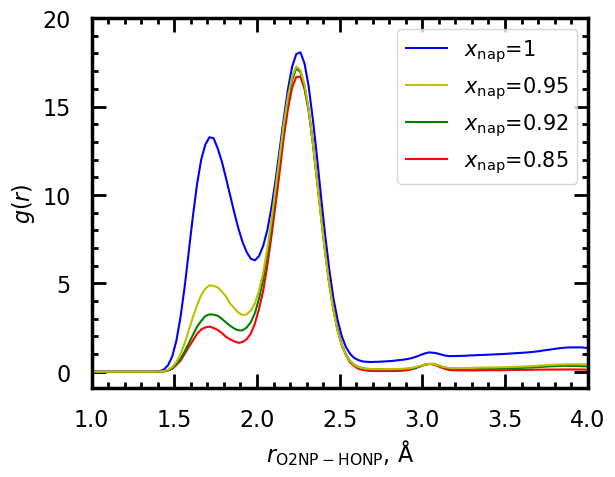
\includegraphics[width=0.4\linewidth]{img/rdf_nap_api_r3.png}}
	\subfloat{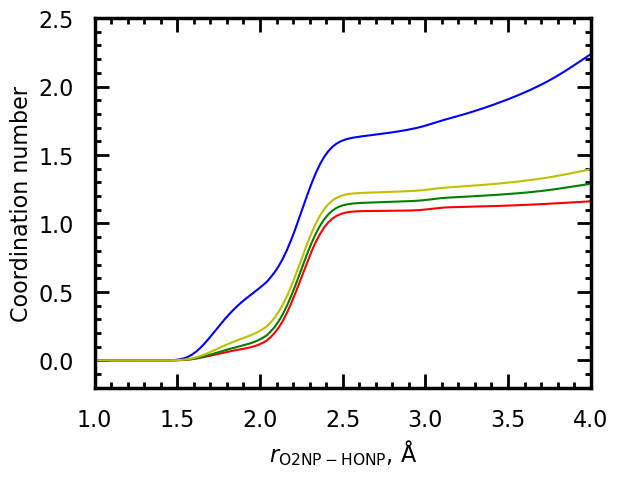
\includegraphics[width=0.4\linewidth]{img/coord_nap_api_r3.png}}\\
	\subfloat{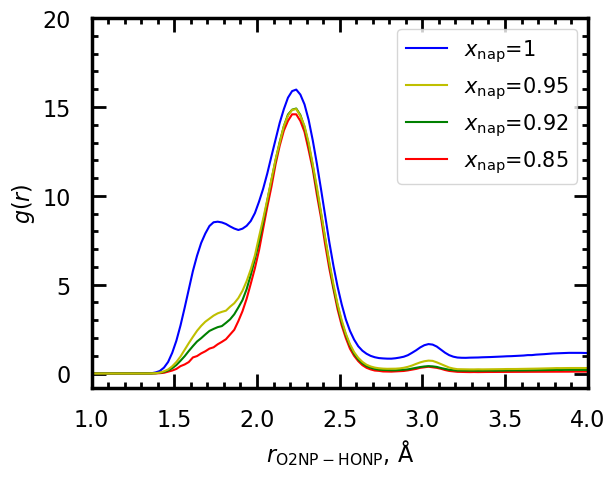
\includegraphics[width=0.4\linewidth]{img/rdf_nap_api_r2.png}}
	\subfloat{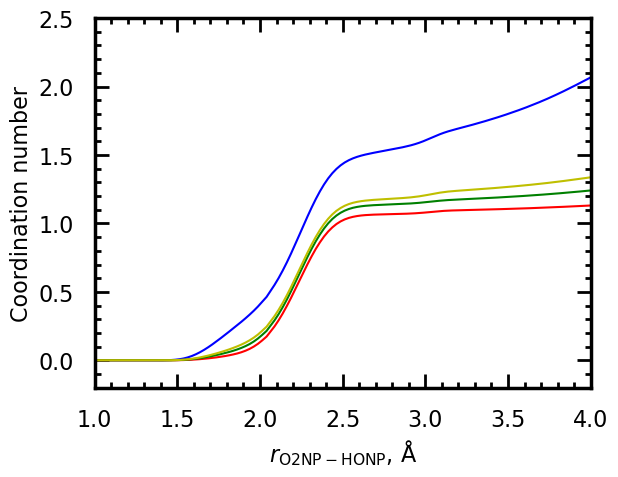
\includegraphics[width=0.4\linewidth]{img/coord_nap_api_r2.png}}
	\vspace{-0.3cm}
	\caption{RDF of the API-API interaction between HONP hydrogen atom and O2NP oxygen atom from COOH group in a mixture of naproxen (nap) and PLA for different concentration normalized on values for pure nap, temperature of 300~K in the left upper corner and 500~K bottom left, coordination numbers on the right.}
	\label{fig:nap_RDF_}
\end{figure}

The RDF of the interaction in carboxyl groups of ibuprofen is shown in Figure \ref{fig:ibu_s_RDF_}. In pure API, the COOH dimer is linked by two hydrogen bonds, corresponding to the first massive peak of the RDF function. This closest contact distance of double bonded COOH dimer is 1.75 \AA. The addition of polymer can disrupt the closest API-carboxyl dimers. With the higher concentration of PLA in the mixture, the height of the first peak is lower. The dominant interaction in mixtures is O-H$\cdots$C looser contact presented at 2.25 \AA. The reason for preferred looser contact in mixtures could be spherical. By the addition of the polymer, the first sphere is partly taken by interactions of hydroxyl hydrogens from API with carbonyl oxygens from PLA which happen at distance 2 \AA, where the minima of API-API RDF function is located. This contact is described further in the PLA-API interaction part. Here, we can observe interesting increase of the third peak at distance 2.95 \AA corresponding to the coordination of second OH group on carbonyl oxygen.

\begin{figure}[H]
	\centering
	\subfloat{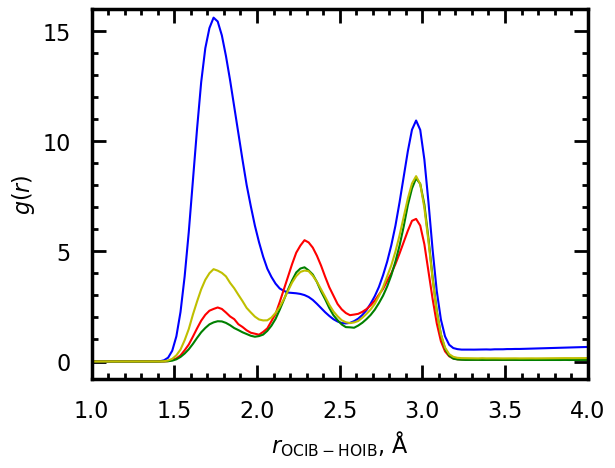
\includegraphics[width=0.4\linewidth]{img/rdf_ibu_s_api_r3.png}}
	\subfloat{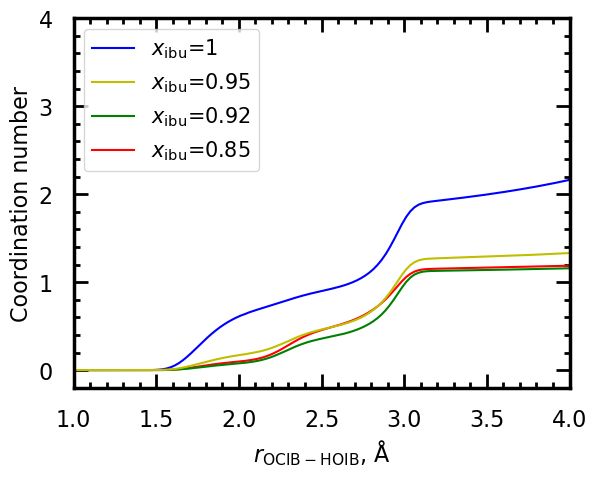
\includegraphics[width=0.39\linewidth]{img/coord_ibu_s_api_r3.png}} \\
	\subfloat{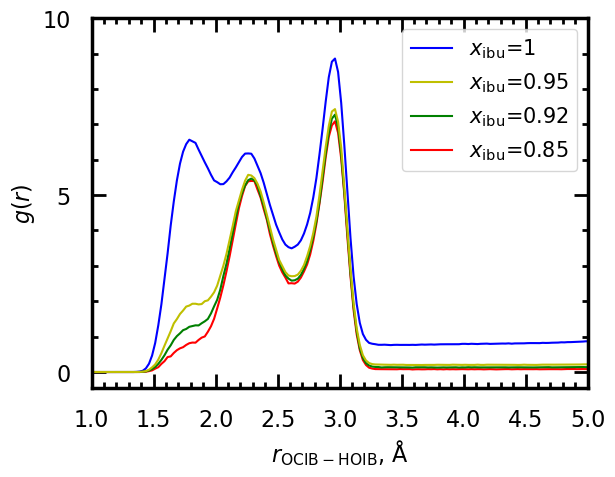
\includegraphics[width=0.4\linewidth]{img/rdf_ibu_s_api_r2.png}}
	\subfloat{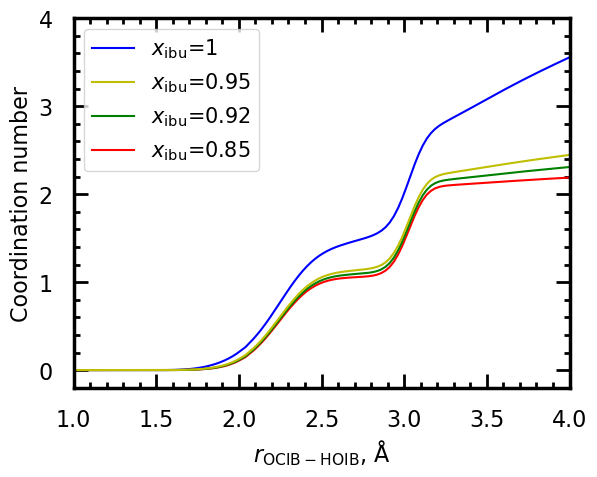
\includegraphics[width=0.39\linewidth]{img/coord_ibu_s_api_r2.png}}
	\vspace{-0.3cm}
	\caption{RDF of the API-API interaction between carboxyl HOIB hydrogen atom and OCIB oxygen atom in a mixture of ibuprofen (ibu) and PLA for different concentration normalized on values for pure ibu, temperature of 300~K in the left upper corner and 500~K bottom left, coordination numbers on the right.}
	\label{fig:ibu_s_RDF_}
\end{figure}

The RDF of the hydrogen bonding interaction of carbamazepine is shown in Figure \ref{fig:cbz_RDF_}. There are two peaks presented, that correspond to interactions of two equivalent hydrogen atoms bonded on nitrogen, each participating the same linking amide-carbonyl dimer with two hydrogen bonds. The closest contact distance N-H$\cdots$O is 2.25 \AA. The shape and signal response of the peaks is similar for neat API and  mixtures for both temperatures. There is almost no change between different concentration of API, meaning that the impact of PLA on the cohesion of carbamazepine in the mixture is very low. 


\begin{figure}[htb]
	\centering
	\subfloat{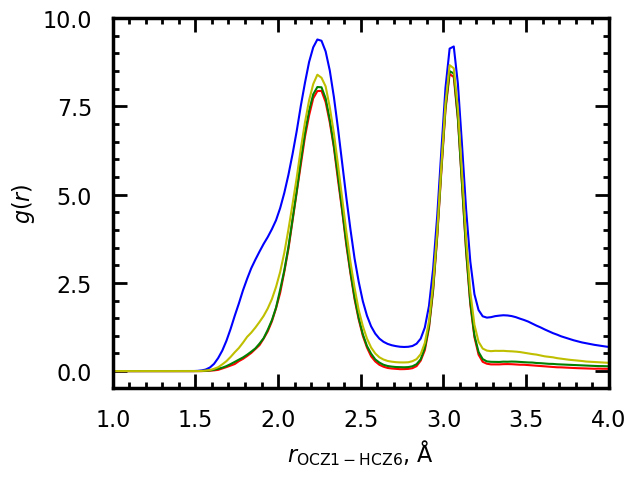
\includegraphics[width=0.41\linewidth]{img/rdf_cbz_api_r3.png}}
	\subfloat{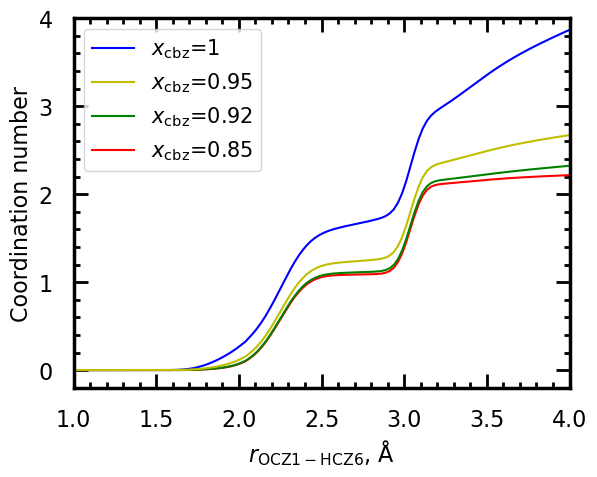
\includegraphics[width=0.39\linewidth]{img/coord_cbz_api_r3.png}}\\
	\subfloat{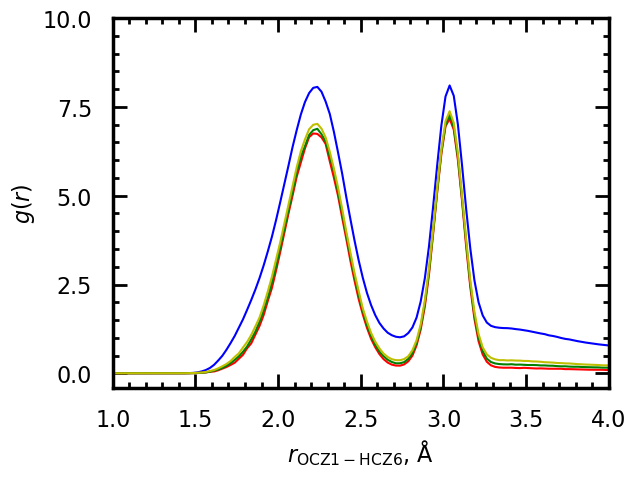
\includegraphics[width=0.41\linewidth]{img/rdf_cbz_api_r2.png}}
	\subfloat{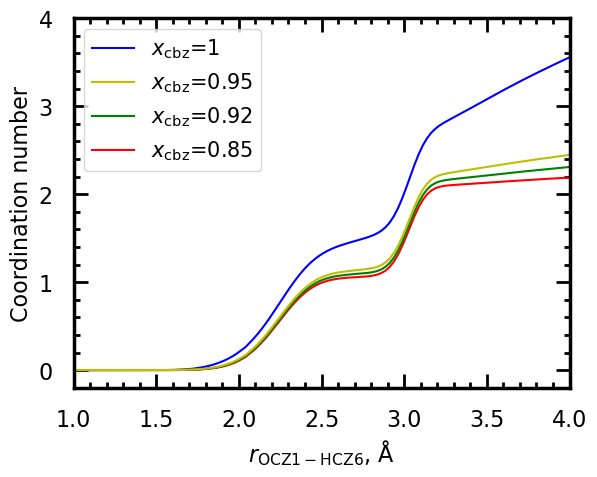
\includegraphics[width=0.39\linewidth]{img/coord_cbz_api_r2.png}}
	\vspace{-0.3cm}
	\caption{RDF of the API-API interaction between HCZ6 hydrogen atom bonded on nitrogen and OCZ1 oxygen atom in a mixture of cbz and PLA for different concentration normalized on values for pure cbz, temperature of 300~K in the left upper corner and 500~K bottom left, coordination numbers on the right.}
	\label{fig:cbz_RDF_}
\end{figure}

\newpage
\textbf{API-PLA interactions}

In this part, we are focusing on the hydrogen bonding between API and PLA. To have a better insight on how the clusters are orientated in space, we performed series of quantum optimizations based on the conformation from simulated trajectories. Optimization of the conformations was performed for each dimer composed of two units long PLA chain and one API molecule using quantum methods in Gaussian\cite{frisch_gaussian16_2016} software by B3LYP functional with the 6-31+g(d,p) basis set with the dispersion correction GD3BJ \cite{smith_revised_2016}. We studied interactions between oxygen (carbonyl and ether bonded) from PLA with hydrogen from API, where API acts as a donor of hydrogen and PLA as its acceptor. The optimized configuration with the studied atom types marked are available in Figure~\ref{fig:contact}.


\vspace{-0.3cm}
\begin{figure}[htb!]
	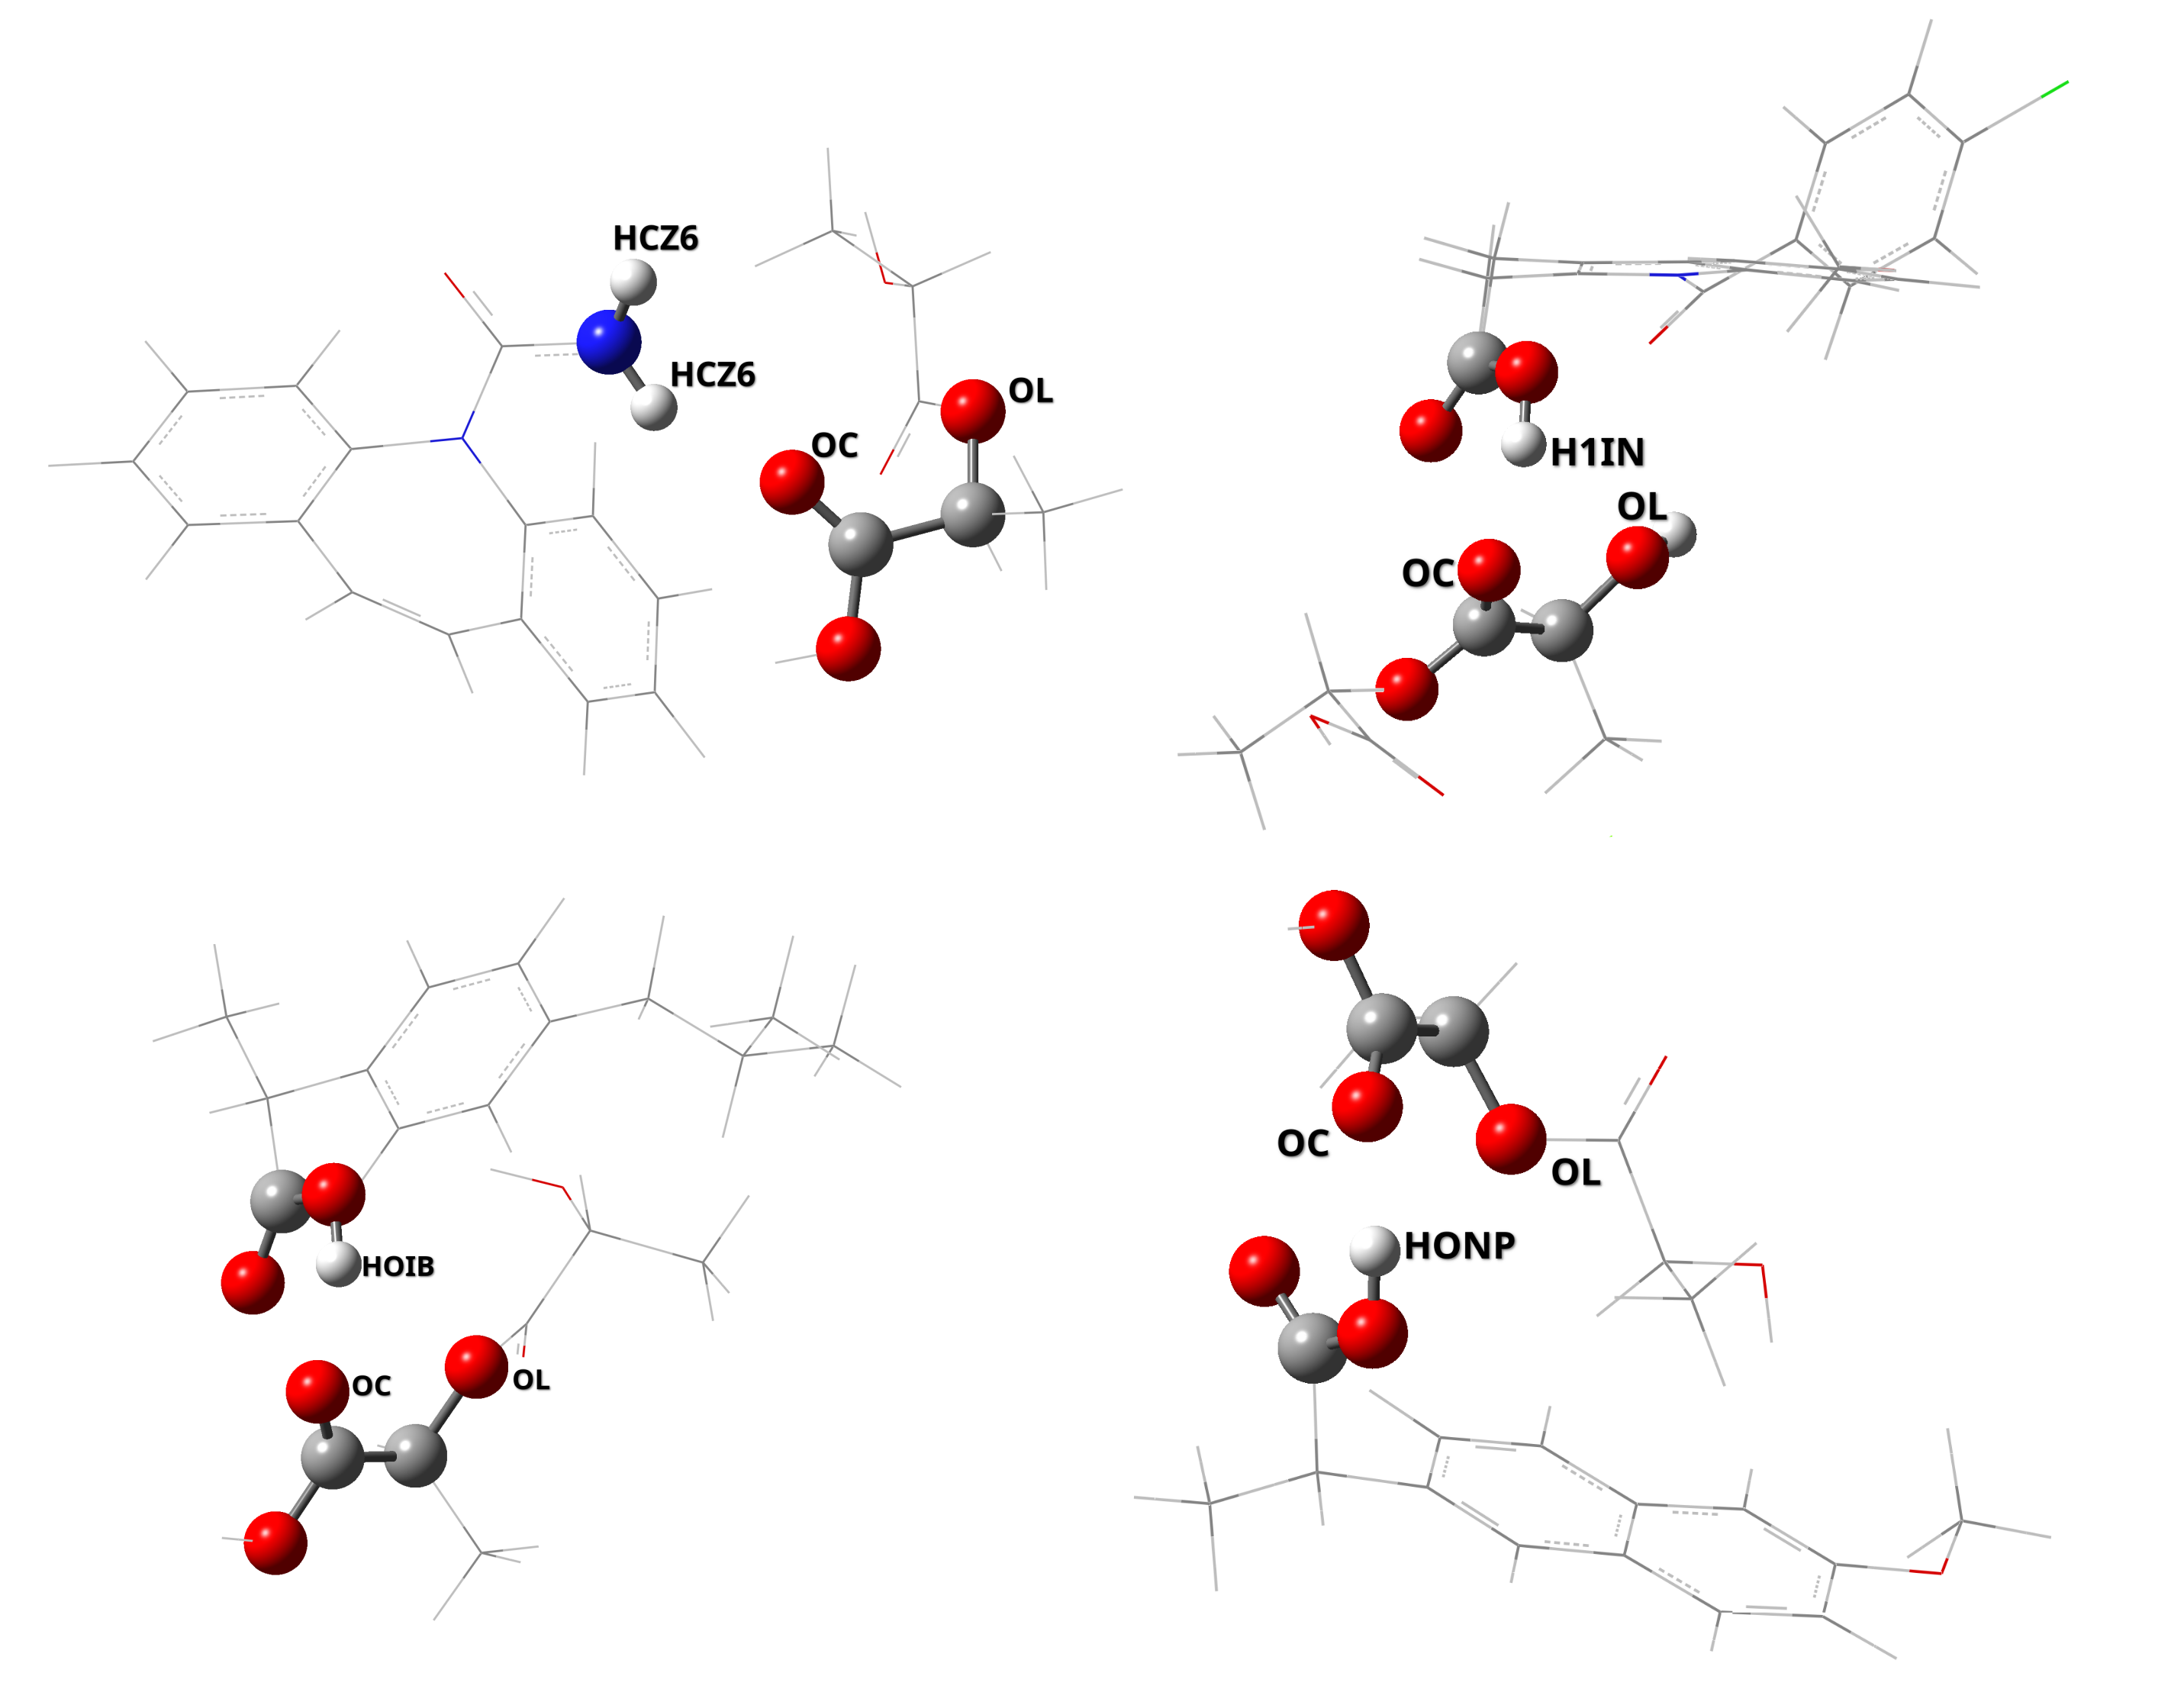
\includegraphics[width=\linewidth]{img/all_pla_api_bp.png} 
	\vspace{-1cm}
	\caption{Visualization of the interaction between hydrogen atom from API and oxygen atom from PLA with marked atom types involved. Carbamazepine (\textbf{top left}), indomethacin (\textbf{top right}), ibuprofen (\textbf{bottom left}) and naproxen (\textbf{bottom right}).}
	\vspace{-0.3cm}
	\label{fig:contact}    
\end{figure}


First, we will discuss the RDF of hydrogen bonding with the carbonyl group from PLA (OC) shown in Figure \ref{fig:carbonyl}. The RDF value converges to one in a long distance for all API-PLA interactions, which is in good agreement with theory. For indomethacine, the amplitude of the peak decreases for lower molar fractions of PLA molecules presented in the mixture. This correspond with the observation for trends in INDO-INDO interactions. The contact distance in cluster obtained from quantum optimization is 1.76 \AA, from MD simulation, we obtained the value of 1.75 \AA.

In case of naproxen, the RDF data show one peak at distance of 1.71? \AA, the value obtained by quantum simulation is 1.76 \AA. The first peak amplitude is lower than for ibuprofen, but slightly higher compared to indomethacine. 

The RDF data for ibuprofen exhibit similar behavior, with slightly higher peak amplitude. For the temperature 300~K, there is a different ordering of heights of the peaks. The peak corresponding to $x_\text{API}=0.85$ is switched with the one corresponding to $x_\text{API}=0.92$. The difference between those peaks is small, but it is strange compared to trend observed in IBU-IBU RDF. The horizontal shift of the peak position is same as for naproxen, the calculated QM value is 1.77 \AA~for IBU.

For carbamazepine, there are two peaks in the RDF function (third row in Figure \ref{fig:carbonyl}) corresponding to two equivalent hydrogens bonded on nitrogen. The peaks corresponding to those interactions are weak, we can see that the intensity of the peaks is really low. Under temperature 300 K, the intensity of the first peak is slightly above one, but for 500 K the first peak is below one, meaning that this interaction occurs less at a small distance than in the rest of the system. The impact of the PLA concentration change is not that visible, especially for higher temperature of 500~K. This also corresponds to what we saw in the CBZ-CBZ interactions. The contact distance value from quantum calculations is 2.01 \AA, which is the same as the distance of the first RDF obtained by MD.


This part is about the hydrogen bonding of oxygen bonded by ether bond in PLA structure and hydrogen from API, that are shown in Figure \ref{fig:ether}. All values also converge to 1 in a long distance for all APIs. Generally, those interactions are much weaker than those with oxygen from carbonyl group. For indomethacine and carbamazepine the value is below one at short distance, with the dimer contact distance obtained from QM 2.55 and 4.19 \AA~respectively. For ibuprofen the order of peaks amplitude for 300~K is also different with the peak for $x_\text{API}=0.92$ having the biggest value. For the temperature of 500~K the change in order is no longer visible. The QM distance between API hydrogen and ether-bonded oxygen in PLA for ibuprofen is 2.48 \AA. For naproxen the QM contact distance is 2.59 \AA. 


\newpage
\begin{figure}[H]
	\centering
	\subfloat{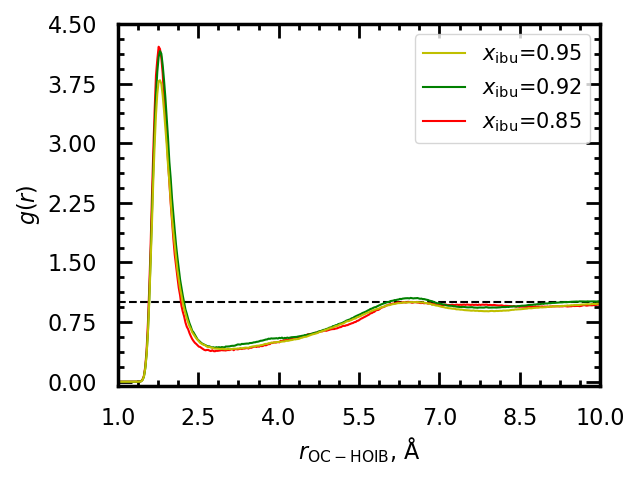
\includegraphics[width=0.5\linewidth]{img/RDF_Coordination_ibu_20_2.png}}
	\subfloat{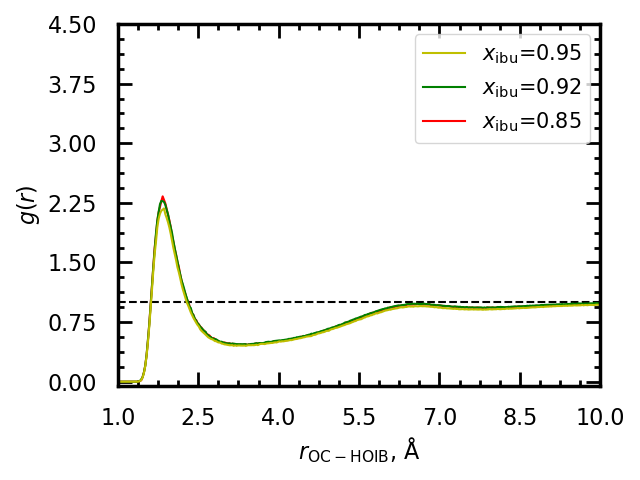
\includegraphics[width=0.5\linewidth]{img/RDF_Coordination_ibu_20_2_r2.png}}\\
	\vspace{-0.2cm}
	\subfloat{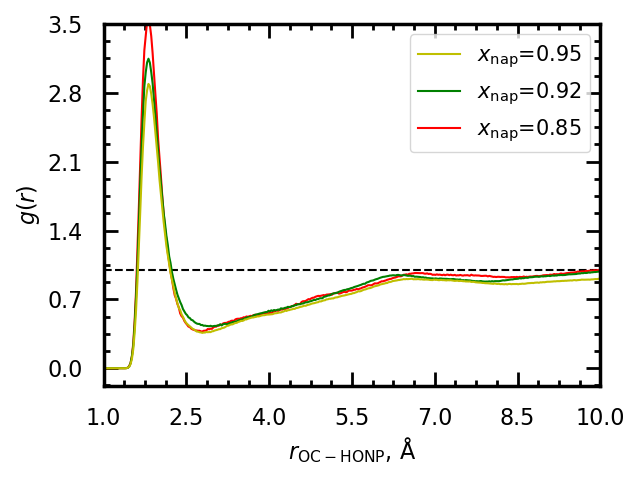
\includegraphics[width=0.5\linewidth]{img/RDF_Coordination_nap_2_31.png}}
	\subfloat{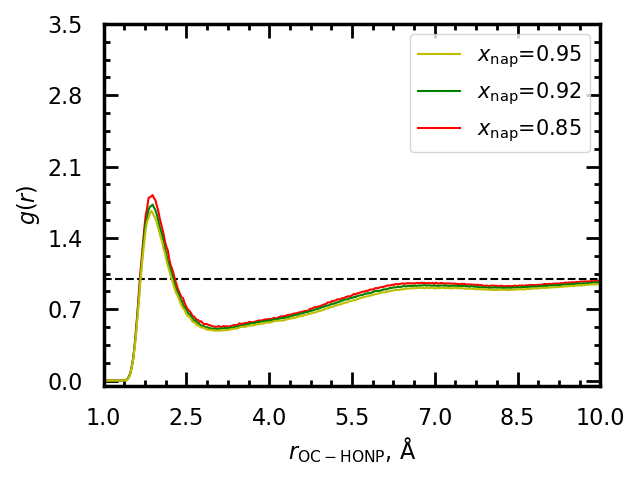
\includegraphics[width=0.5\linewidth]{img/RDF_Coordination_nap_2_31_r2.png}}\\
	\vspace{-0.2cm}
	\subfloat{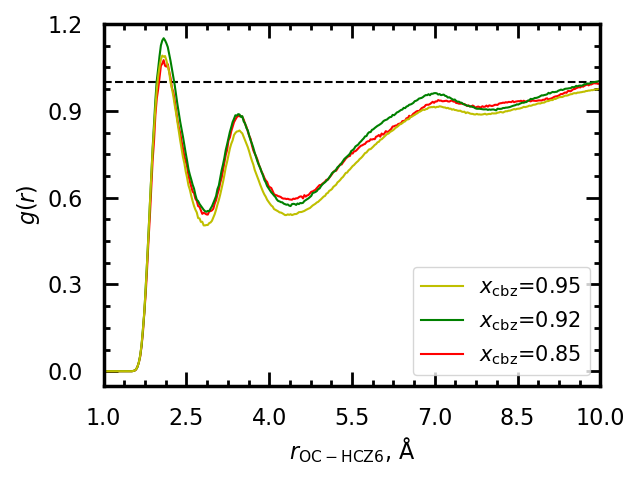
\includegraphics[width=0.5\linewidth]{img/RDF_Coordination_cbz_2_27.png}}
	\subfloat{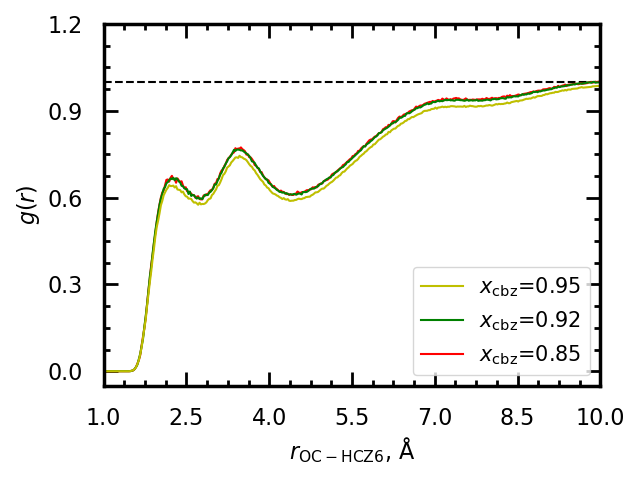
\includegraphics[width=0.5\linewidth]{img/RDF_Coordination_cbz_2_27_r2.png}}\\
	\vspace{-0.2cm}
	\subfloat{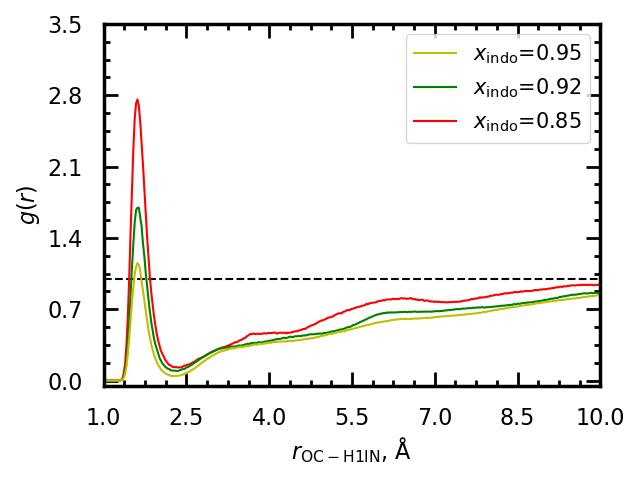
\includegraphics[width=0.5\linewidth]{img/RDF_Coordination_indo_2_36.png}}
	\subfloat{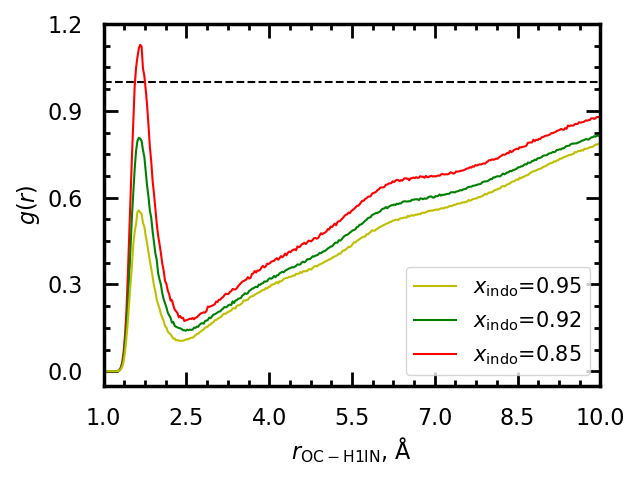
\includegraphics[width=0.5\linewidth]{img/RDF_Coordination_indo_2_36_r2.png}}
		\vspace{-0.2cm}
	\caption{Radial distribution functions of the interaction between hydrogen atoms participating at hydrogen bond and the oxygen atom from carbonyl groups in PLA. First row - IBU, second row - NAP, third row - CBZ and fourth row - INDO, temperature 300~K on the left and 500~K on the right.}
	\label{fig:carbonyl}
\end{figure}

\newpage
\begin{figure}[H]
	\centering
	\subfloat{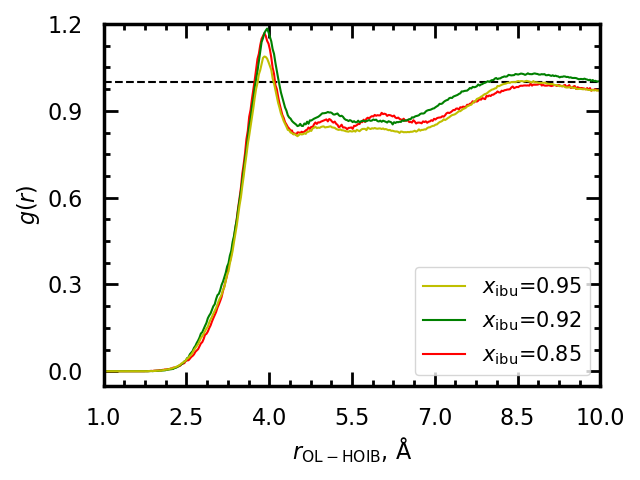
\includegraphics[width=0.5\linewidth]{img/RDF_Coordination_ibu_20_6.png}}
	\subfloat{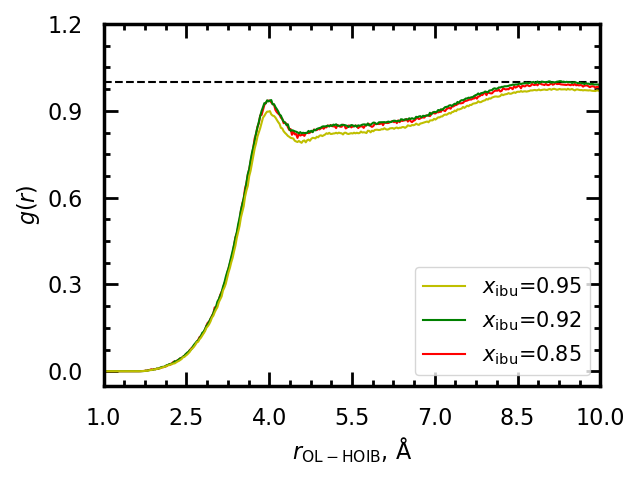
\includegraphics[width=0.5\linewidth]{img/RDF_Coordination_ibu_20_6_r2.png}}\\
	\vspace{-0.2cm}
	\subfloat{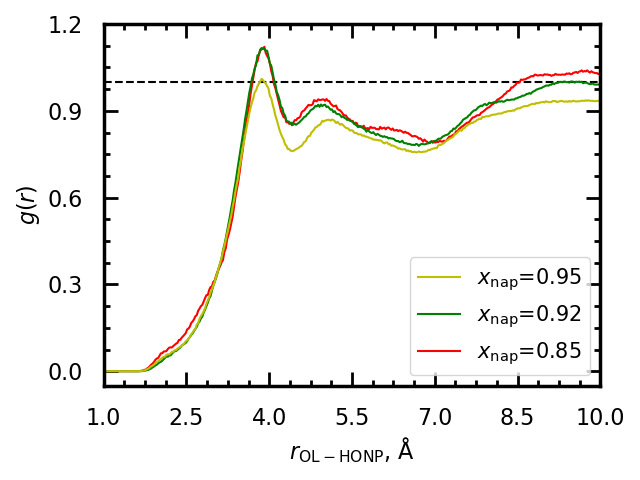
\includegraphics[width=0.5\linewidth]{img/RDF_Coordination_nap_6_31.png}}
	\subfloat{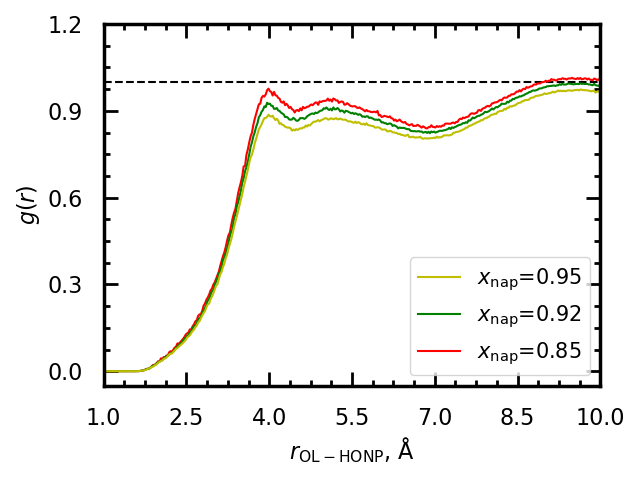
\includegraphics[width=0.5\linewidth]{img/RDF_Coordination_nap_6_31_r2.png}}\\
	\vspace{-0.2cm}
	\subfloat{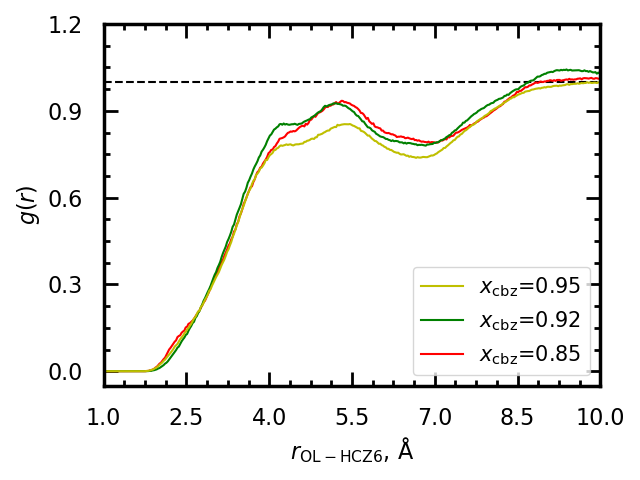
\includegraphics[width=0.5\linewidth]{img/RDF_Coordination_cbz_6_27.png}}
	\subfloat{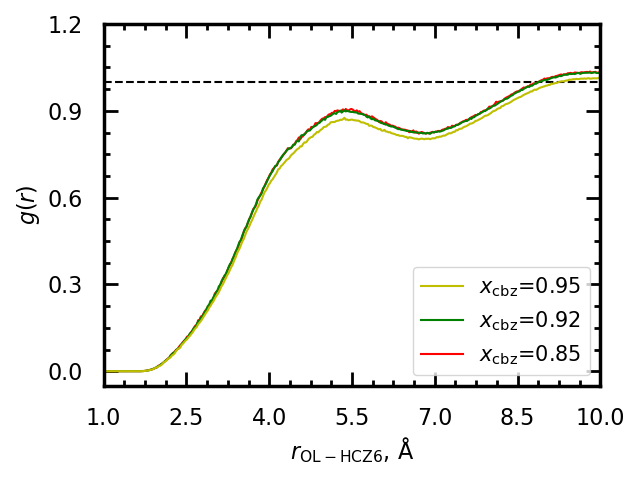
\includegraphics[width=0.5\linewidth]{img/RDF_Coordination_cbz_6_27_r2.png}}\\
	\vspace{-0.2cm}
	\subfloat{\includegraphics[width=0.5\linewidth]{img/RDF_Coordination_indo_36_6.png}}
	\subfloat{\includegraphics[width=0.5\linewidth]{img/RDF_Coordination_indo_36_6_r2.png}}
	\vspace{-0.2cm}
	\caption{Radial distribution functions of the interaction between hydrogen atoms participating at hydrogen bond and the oxygen atom bonded by ether bond in PLA. First row - IBU, second row - NAP, third row - CBZ and fourth row - INDO, temperature 300~K on the left and 500~K on the right.}
	\label{fig:ether}
\end{figure}

\newpage
\subsubsection{Diffusion coefficients}
The MSDs were sampled from the 10~ns long simulation runs every 1000 fs (integration step 1 fs). At each sampled time step, obtained MSD data were averaged over all API molecules and then plotted as a function of the simulation time. The MSD dependencies were then interpolated by linear functions and related self-diffusivities of the API in the mixtures were evaluated from the slope of the line using the following Equation \ref{eq:D} obtained by modifying the Einstein equation from the theoretical part.
\vspace{-0.25cm}
\begin{equation}\label{eq:D}
	D_{\text{API}} = \frac{a}{6}, 
\end{equation}
where $D$ is the diffusion coefficient, $a$ is the slope interpolating the linear MSD regime.

The MSD data for APIs in mixtures with PLA for $T$=500~K are plotted in Figure \ref{fig:msd_r2}. The data of carbamazepine show that with increasing API concentration, the diffusivity of API molecules also increases. The polymer is able to attenuate the diffusivity of CBZ molecules in the mixture when compared to neat amorphous CBZ. This behavior could stem from the intermolecular interactions between CBZ-PLA, but this trend was not visible in the analysis of RDFs. However, the dominating factor determining the diffusivity at higher temperatures is the shape of the molecules and sterical factors, when immobile polymer impedes motion of the CBZ molecules. This could be the case why PLA slows down relatively big carbamazepine molecules, even though any strong interaction between CBZ-PLA were not observed. 

For naproxen, it seems that there is no significant variation of MSD among different concentrations of mixtures, but the diffusivity is again slightly higher for neat API. Here we can describe it by forming specific NAP-PLA interactions and linking NAP to PLA molecule, the diffusivity of which is lower. This is in agreement with the RDF analysis. We should also have a look at the data for lower temperature.

For ibuprofen, there is a significant difference between mobility of neat IBU and its mixture, note the values on vertical axis. This could be a result of very strong IBU-PLA interactions that are formed in the mixtures. Analysis of RDF showed that ibuprofen had the strongest IBU-PLA interactions among the considered APIs.

The situation for indomethacine is completely different, the MSD values of neat INDO are much lower. For neat API, the mobility is really low compared to mixtures with PLA. This behaviour seems strange in context of other API. The reason could be that in pure INDO, there are really strong INDO-INDO interactions that decrease the mobility of its molecules. The number of those interactions is lower after adding the polymer. This was visible from the corresponding RDFs for INDO-INDO interactions, where indomethacine had the strongest intermolecular interactions decreasing with INDO concentration. For this to be true, the diffusivity of pure PLA must be greater than that of pure INDO. Self-diffusivities were evaluated from the above data and plotted in Figure \ref{fig:d}. 

\begin{figure}[]
	\centering
	\subfloat{\includegraphics[width=0.4\linewidth]{img/msd_cbz_api_r2.png}}
	\subfloat{\includegraphics[width=0.4\linewidth]{img/msd_nap_api_r2.png}}\\
	\subfloat{\includegraphics[width=0.4\linewidth]{img/msd_ibu_s_api_r2.png}}
	\subfloat{\includegraphics[width=0.4\linewidth]{img/msd_indo_api_r2.png}} 
	\caption{MSD from simulations under 500 K, carbamazepine (\textbf{top left}), naproxen (\textbf{top right}), ibuprofen (\textbf{bottom left}) and indomethacin (\textbf{bottom right}).}
	\label{fig:msd_r2}    
\end{figure}

\newpage


%The data reveal that in pure liquid carbamazepine the diffusion is faster than in naproxen. For higher temperatures, the main factor affecting diffusion is the shape of the molecules, not the strength of the intermolecular interactions. This is caused because the kinetic energy is higher than the potential for higher temperatures.
\begin{figure}[htb!]
	\centering
	\includegraphics[width=0.6\linewidth]{img/d.png} 
	\caption{Self-diffusivities ($D$) for carbamazepine, naproxen, ibuprofen and indomethacine as a function of their concentration in the mixtures, temperature 500 K. Data shown in logarithmic scale, artificial small horizontal axis offset is used for better readability}
	\label{fig:d}    
\end{figure}  

MSD was also evaluated at a lower temperature of 300 K, Figure \ref{fig:msd_r1}. For carbamazepine, there is no visible variation of changed diffusivity for different concentrations, from that we can definitely say, that addition of PLA has minimal effect on the behavior of CBZ. The situation of of naproxen is similar, we cannot determine any important difference between the different concentrations in order of magnitude of simulation error. For ibuprofen, the situation is the same as for 500~K, the addition of PLA will result in lower diffusivity of IBU molecules in the mixture. For indomethacin, there is also no visible trend, the diffusivity of the mixture with the least amount of PLA is somewhat higher. The diffusivity of INDO at 300~K is about the same as for PLA, this is the reason for no change in diffusivity by adding the polymer to neat INDO. 


\begin{figure}[H]
	\centering
	\subfloat{\includegraphics[width=0.4\linewidth]{img/msd_cbz_api_r3.png}}
	\subfloat{\includegraphics[width=0.4\linewidth]{img/msd_nap_api_r3.png}}\\
	\subfloat{\includegraphics[width=0.4\linewidth]{img/msd_ibu_s_api_r3.png}}
	\subfloat{\includegraphics[width=0.41\linewidth]{img/msd_indo_api_r3.png}} 
	\caption{MSD from simulations under 300 K, carbamazepine (\textbf{top left}), naproxen (\textbf{top right}), ibuprofen (\textbf{bottom left}) and indomethacin (\textbf{bottom right}).}
	\label{fig:msd_r1}    
\end{figure}

\subsubsection{Glass transition temperature}
The glass transition temperatures of the mixtures were evaluated from the fast (30~K ns$^{-1}$) non-equilibrium gradual cooling runs by fitting a hyperbola to the temperature-density data. The whole methodology is described in the paper written by Alzate-Vargas et al.\cite{alzate-vargas_uncertainties_2018}, the main equation of the fit is Equation \ref{eq:fit}

\begin{equation}\label{eq:fit}
	\rho(T)=\rho_0-a\left(T-T_0\right)-b\left[\frac{1}{2}\left(T-T_0\right)+\sqrt{\frac{\left(T-T_0\right)^2}{4}+e^c}\right],
\end{equation}

where $T_0, \rho_0, a, b, c$ are initial parameters.

\vspace{-0.3cm}
The representative data sets used for determination of $T_\textbf{g}$ with the hyberbolic fit are displayed in Figure \ref{fig:tg_evaluation} for each API. The data obtained correspond to the cooling run which was initiated from the configuration reached after the mixture spent 2 ns at 800~K of the 5~ns long simulation. \vspace{-0.5cm}
\begin{figure}[H]
	\centering
	\subfloat{\includegraphics[width=0.5\linewidth]{img/cbz_tg_tag.png}}
	\subfloat{\includegraphics[width=0.5\linewidth]{img/nap_tg_tag.png}}\\
	\subfloat{\includegraphics[width=0.5\linewidth]{img/ibu_s_tg_tag.png}}
	\subfloat{\includegraphics[width=0.5\linewidth]{img/indo_tg_tag.png}} 
	\vspace{-0.2cm}
	\caption{Determination of the glass transition temperature $T_\text{g}$ of mixture with API concentration of $x_\text{API}$=0.85 by the non-equilibrium hyperbola fit method, second data set. Two vertical gray lines correspond to the different values of $c$ parameter from hyperbola fit (for the line passing broken cyan line $c=-\infty$) Carbamazepine (\textbf{top left}), naproxen (\textbf{top right}), ibuprofen (\textbf{bottom left}) and indomethacin (\textbf{bottom right}).}
	\label{fig:tg_evaluation}    
\end{figure}


If there is a clearly visible bend in the data for our system (glass transition happens fast at once), the determination of $T_\textbf{g}$ is more reliable and has less uncertainty. The vertical gray lines (corresponding to different $c$ parameters from hyperbola fit equation) are also closer with respect to the value on horizontal axis. This can be shown on the example of CBZ. If the transition between the liquid and the glassy state is not this sharp, it is harder to determine $T_\textbf{g}$ and the associated uncertainty of the resulting value is higher. This is evident in the example of indomethacin where the gray lines are further away and the order of magnitude larger uncertainties are visible than for other APIs.

The cooling of the system from liquid can lead to "frozen" conformations of amorphous solid state, more independent simulated runs starting from different configurations must be performed to evaluate $T_\text{g}$ with the information about its uncertainty as it was described in the methods section. We used data from 5 ns long simulation run at the temperature of 800~K, which is high enough to erase any conformational preferences and thermal history. We performed 5 simulations starting from different initial states. The value for each run and its uncertainty is given in Figure \ref{fig:results_tg}. 

\begin{figure}[htb!]
	\centering
	\subfloat{\includegraphics[width=0.5\linewidth]{img/results_tg.png}}
	\subfloat{\includegraphics[width=0.5\linewidth]{img/results_tg_indo.png}}
	\vspace{-0.2cm}
	\caption{Calculated glass transition temperatures $T_\text{g}$ of mixtures composed from API and PLA with concentration of $x_\text{API}$=0.85 starting from 5 different configurations, mean values averaged over the five independent runs plotted by dashed lines for each API with their uncertainties, point 6. Artificial small horizontal axis offset is used for results of individual API for better readability.}
	\label{fig:results_tg}    
\end{figure}  



The Table \ref{tab:Tg_mix} shows the mean value of $T_\text{g}$ with the uncertainty for the mixtures of API and PLA with $x_\text{API}=0.85$ obtained from 5 runs from different starting conformations. The calculation of the uncertainties is shown in Equation \ref{eq:sigma}. The $T_\textbf{g}$ values of neat APIs, which were obtained from MD simulations by Červinka et al. \cite{cervinka_structure_2021} using the same force field models as in this work, are shown for comparison. The whole description of their methodology could be found there. 

\begin{equation}\label{eq:sigma}
	\sigma_{T_{\text{g}}^\text{MIX}} = \sum_{runs} \sigma_{T_{\text{g}}^\text{}}^2 + \sigma_{T_{\text{g}}^\text{worst}}^2
\end{equation}

where $\sigma_{T_{\text{g}}^\text{}}^2$ is the uncertainty of the individual run and  $\sigma_{T_{\text{g}}^\text{worst}}^2$ is the biggest uncertainty of all runs for each API.

\begin{table}[htb!]
	\caption{Calculated glass transition temperatures $T_\text{g}^\text{MIX}$ of mixtures composed from API and PLA with concentration of $x_\text{API}$=0.85 and their standard uncertainties, data for $T_\text{g}^\text{NEAT}$ of neat APIs obtained from \cite{cervinka_structure_2021}.}
	\centering
	\begin{tabular}{lccc} \toprule
		{\textbf{API}} & {\textbf{\boldmath{$T_{\text{g}}^\text{MIX}$}}} & \textbf{{\boldmath{$\sigma_{T_{\text{g}}^\text{MIX}}$}}} &
		\textbf{\boldmath{$T_{\text{g}}^\text{NEAT}$}}\\
		\midrule
		carbamazepine  & 370 & 4 & 384\\		
		naproxen   & 370 & 9 & 343\\
		ibuprofen  & 363 & 4 & 295\\
		indomethacin  & 408 & 78 & 388\\
		PLA & - & - & 337\\
		\bottomrule
	\end{tabular}
	\label{tab:Tg_mix} 
\end{table} 


The higher diffusivity, the faster molecular motion is observed leading to a lower value of $T_\text{g}$ and different kinetics of an glass transition. When the material maintain high diffusivity even at lower temperatures, it tends to crystallize more easily. However, the materials with low diffusivity are having troubles with crystallization and tend to form supercooled liquids or glassy states, which is desired for our application use. For mixtures with a visible decrease of diffusivity in MSD plots after adding polymer, we would expect a higher $T_\text{g}$ value of the mixture than $T_\text{g}$ of neat API. This is true in case of ibuprofen, where the $T_\textbf{g}$ value increases significantly for its mixture. This is a good example of stabilization of the IBU-PLA mixture, which exhibited strong IBU-PLA interactions. The similar, but weaker effect could be seen in case of naproxen too.

The opposite trend should be visible for indomethacin, where the $T_\textbf{g}$ value should be lower for the mixture than for neat INDO. However, the uncertainty of the INDO $T_\textbf{g}$ value for mixture is huge, also relatively compared to other APIs. Within the interval of uncertainty, the $T_\textbf{g}$ values for neat INDO and its mixture are comparable. 

For carbamazepine, the $T_\textbf{g}$ value for the mixture is between the values for neat API and PLA. This is not in correspondence with the previous description. Carbamazepine exhibited a higher decrease of the diffusivity between its mixture and neat state than naproxen. On the other hand, in the mixtures of CBZ almost none interactions with PLA were presented. The mixture of CBZ behave almost ideally, having the $T_\textbf{g}$ in between values for neat PLA and CBZ. The determination of the glass-transition temperature by this method is not that accurate, this could be seen in the data for the mixture of indomethacine, where the uncertainty was high. However, we were still able to observe some qualitative trends.
